% Copyright (C) 2013-2014 Shanghai Experimental School T.M. Mathematical Modeling Group. All rights are reserved!
% This is the paper, Curriculum Schedule Optimization, Version 3.4 (Final-2), Date 2014-06-04.
% The file is distributed only for people of the T.M. Mathematical Modeling Group.
% Permission for any other use of this file must be obtained in writing
% from the copyright holders and authors (Yiwei Tan, Yifan Cao, Sichong Zhao).
% !TeX program = xelatex
% !TeX encoding = UTF-8
% !TeX spellcheck = en_US
\documentclass[a4paper]{article}
\usepackage{xltxtra,fontspec,xunicode}
\usepackage{xeCJK}
\xeCJKsetup{CJKspace=true}
\setCJKmainfont[BoldFont=SimHei,ItalicFont=KaiTi]{SimSun}
\setlength{\parindent}{2em}
\setlength{\hoffset}{-30pt}
\setlength{\voffset}{-20pt}
\setlength{\textwidth}{405pt}
\setlength{\textheight}{670pt}
\usepackage{hyperref}
\hypersetup{unicode,bookmarksnumbered,bookmarksopen,breaklinks,colorlinks,linkcolor=black,citecolor=black,urlcolor=black}
\usepackage{fancyhdr}
\pagestyle{fancy}
\fancyhf{}
\usepackage{lastpage}
\usepackage[title,titletoc,header]{appendix}
\usepackage{amsmath,amsfonts,amssymb}
\usepackage{graphicx,xcolor}
\usepackage{float}
\usepackage[labelsep=quad]{caption}
\usepackage{overpic}
\usepackage{tikz}
\usepackage{flowchart}
\usepackage{listings}
\usepackage{forloop}
\lstset{
language=Matlab,
breaklines=true,
columns=flexible,
basicstyle=\ttfamily,
keywordstyle=\color{blue}
}
\usepackage{isomath} % ISO 数学排版标准
\renewcommand{\vec}{\vectorsym} % ISO: 数学模式下使用 \vec{A} 打出向量 A (倾斜粗体)
\renewcommand{\matrix}{\matrixsym} % ISO: 数学模式下使用 \matrix{A} 打出矩阵 A (倾斜粗体)
\newcommand{\tensor}{\tensorsym} % ISO: 数学模式下使用 \tensor{A} 打出张量 A (倾斜无衬线粗体)
\newcommand{\me}{\mathrm{e}} % ISO: 数学模式下使用 \me 打出科学常数 e (直立体)
\newcommand{\mi}{\mathrm{i}} % ISO: 数学模式下使用 \mi 打出虚数单位 i (直立体)
\newcommand{\dif}{\mathrm{d}} % ISO: 数学模式下使用 \dif 打出微分算子 d (直立体)
\DeclareSymbolFont{lettersA}{U}{txmia}{m}{it}
\DeclareMathSymbol{\piup}{\mathord}{lettersA}{"19} % ISO: 数学模式下使用 \piup 打出圆周率 pi (直立体)
\DeclareSymbolFont{largesymbolsA}{U}{esint}{m}{n}
\DeclareMathSymbol{\ointop}{\mathop}{largesymbolsA}{'013}\def\oint{\ointop\nolimits} % 数学模式下使用 \oint 打出曲线环积分号
\DeclareMathSymbol{\oiintop}{\mathop}{largesymbolsA}{'015}\def\oiint{\oiintop\nolimits} % 数学模式下使用 \oiint 打出曲面环积分号
\setcounter{secnumdepth}{5}
\setcounter{tocdepth}{5}
% 以下是特殊序号用计数器(2-4级)
\newcounter{verytwo}[section]
\newcommand{\verytwo}{\stepcounter{verytwo}\noindent\textbf{\thesection.\arabic{verytwo}}\quad}
\newcounter{verythree}[subsection]
\newcommand{\verythree}{\stepcounter{verythree}\noindent\textbf{\thesubsection.\arabic{verythree}}\quad}
\newcounter{veryfour}[subsubsection]
\newcommand{\veryfour}{\stepcounter{veryfour}\noindent\textbf{\thesubsubsection.\arabic{veryfour}}\quad}
\renewcommand{\headrulewidth}{0.75pt}
\renewcommand{\baselinestretch}{1.2}
\renewcommand{\contentsname}{目\quad 录}
\renewcommand{\refname}{参考文献}
\renewcommand{\figurename}{\bf 图}
\renewcommand{\tablename}{\bf 表}
\renewcommand{\appendixname}{附录}
\begin{document}
\lhead{\bf 第\,\thepage\,页, 共\,\pageref{LastPage}\,页}
\chead{\bf 上海市实验学校课表评价与优化系统}
\rhead{\bf Group 1}
\title{\bf 上海市实验学校课表评价与优化系统}
\author{谈易伟\and 曹逸凡\and 赵思翀}
\date{\number\year\,年\,\number\month\,月\,\number\day\,日}
\maketitle
\thispagestyle{empty}
\section*{\hfil 摘\quad 要}
\addcontentsline{toc}{section}{摘要}
 课程安排是提高学生学习效率与成绩的重要因素. 在这篇论文中, 我们的目的是为上海市实验学校设计一个更优的课表, 让这个课表能够使学生的听课效率, 教师的教课效率与成绩、升学率等得到提高.\par
 首先, 我们对现有的课表进行了收集与分析. 我们对课表中的一些限定条件进行了总结, 例如每节课的长度以及某些课程的特定安排等.\par
 之后, 我们对各个课程的重要程度进行了定义. 很明显的, 将所有课程看成是一样重要是粗糙而不合理的, 所以我们以现行的制度为基础, 为所有课程设计了从\,1\,到\,6\,的六级重要程度. 首先, 语数英的重要程度为\,5, 物理与化学为\,3, 其他课程为\,1. 基于现行的会考制度, 我们又对本年级的会考科目进行了加一的处理, 使得各个年级的特点得以突出.\par
 接着, 我们建立了状态转移模型. 学生的学习效率毫无疑问是与他们的听课效率息息相关的. 首先, 我们将学生的听课效率定为两类, 优良与低下. 我们又假设在一天初始时所有学生的状态都为优良, 在矩阵中的表现即为第一列都为\,1, 建立了一个\,$2\times2$\,的初始矩阵. 之后, 我们又建立了状态转移概率的矩阵. 在此矩阵中, 我们通过敏感度分析得出了各个状态之间相互转移的概率, 通过不断与初始矩阵相乘来计算每一节课处于各个状态的学生的比例. 其次, 我们又假设在午休之后有一定比例的学生回归满状态, 与上午课程无关, 再进行下午的状态分析. 接着, 我们又建立了一个\,$3\times3$\,的矩阵, 将学生的状态细分为优良, 低下与萎靡 (即毫无学习能力, 例如上课睡觉等), 使得模型更加真实可靠. 在优化模型中, 我们具体分析了学生的听课效率, 对课程进行了文理性分析, 又对体育课做了特殊的处理.\par
 在下一个模型中, 我们基于上一个模型所给出的学生状态与重要程度对课表进行了打分. 我们分别对\,$2\times2$\,与\,$3\times3$\,的矩阵进行了打分, 即求课程重要程度与学生状态比例的乘积之和, 以计算学生的总听课效率. 之后, 我们又建立了老师教课效率模型. 在此模型中, 我们对教师的授课状态同样做了状态转移模型, 以计算每一节课教师的授课效率. 之后, 我们将教师的授课效率与学生的听课效率结合在一起, 通过\,Douglas\,生产函数计算了更准确的学生学习效果.\par
 接着我们对现行课表进行了上述的处理, 再将其与高一以来的考试成绩对比, 发现其有较高的吻合度, 验证了我们模型的准确性.\par
 之后, 我们设计了计算机模型, 通过程序来进行上述几个模型的计算, 得出了最优课表并同时进行了敏感度分析. 我们得出不考虑会考科目对现行课表的平均优化率为\,2.308\%, 考虑会考科目的平均优化率为\,4.135\%. 在加入了敏感度分析与优化模型后的平均优化率为\,6.122\%.\par
 接着, 我们又将一天\,9\,节课为基础进行了优化. 再将自修课定义并加入状态转移模型后, 我们得到了新的\,9\,节课的课表. 9\,节课课表对于原课表的平均优化率为\,20.765\%. 在另一种\,9\,节课模型中, 我们得出的平均优化率为\,6.484\%. 最后, 我们也将吃饭后的学习效率加入了优化.\par
 最后, 我们将现行课表进行优化后的综合优化率大约为\,6.2\%\,左右, 对学生的学习效果有了可观的提升.
\clearpage
\tableofcontents
\clearpage
\section{引言}
 本文主要研究的是上海市实验学校初高中的课程安排. 虽然现在的课程安排已经较完善, 但是结合亲身经历, 发现教师与学生都对现在的课程有所不满. 例如, 老师对连续教课及课程过于分散导致自己活动时间较少感到不满, 再比如许多学生在下午上课时感到疲倦, 接受效率低, 这些都是我们需要解决的问题. 通过重新安排、优化课程表, 我们才可以使学生及老师都能够获得最高的效率, 有效提高教师的授课效率及学生的接受效率.
 本文通过使用马尔科夫链建立学生与老师的状态模型得出最优安排. 我们接着优化了许多特殊课程与设定, 例如高三的优化, 创新班的优化, 以及特需课程、社团课等的优化.
\vspace{2cm}
\section{总假设}
 \verytwo 本文只考虑现行高考制度下的课表改革, 并且只选取了我们本校的高一年级进行具体的打分与优化.\par
 {\it 鉴于考虑大范围的课表优化在时间上的可行性不强, 又我们均为高一学生, 对于高一课程设置与老师安排较为熟悉, 故本文只选取了我校高一年级作为考察对象.}\par
 \vspace{2mm}
 \verytwo 本文假设了学生上课效率与学生成绩呈正相关, 通过学生的成绩来衡量课表的优劣.\par
 {\it 上课是学生学习的重要组成部分, 而其余诸如课外辅导等灵活度太强, 且本身与课表优化关系不大, 故本文就不一一考虑.}\par
 \vspace{2mm}
 \verytwo 本文假设学校的指定课程不纳入分析与整改的范围内.\par
 {\it 这些指定课程大多为我校特色课程或代表性课程, 在全市范围内可比性不强, 不能进行合理的考量与分析, 故不将其列入范围内.}\par
 \vspace{2mm}
 \verytwo 本文不把早自修纳入考虑范围内.\par
 {\it 早自修安排相对固定, 所以课程调整中早自修基本不会造成任何影响, 故不把它纳入考虑范围内.}
\clearpage
\section{准备模型}
 \subsection{高一现有课表整理}
  我们依据高一现有的课程表对于所上的科目及每门科目每周的数目进行了统计, 得到了以下表格.
  \begin{table}[H]
  \centering
  \begin{tabular}{|l|c|c|}
  \hline
  \bf 课程 & \bf 平行班 & \bf 创新班\\\hline
  语文 & 5 & \bf 4\\\hline
  数学 & 5 & \bf 4\\\hline
  英语 & 4 & \bf 3\\\hline
  物理 & 3 & 3\\\hline
  化学 & 3 & 3\\\hline
  政治 & 2 & 2\\\hline
  历史 & 2 & 2\\\hline
  地理 & 3 & 3\\\hline
  TFT & 1 & 1\\\hline
  TFT\,英语 & 1 & 1\\\hline
  体育 & 2 & 2\\\hline
  活动 & 1 & 1\\\hline
  信息科技 & 2 & 2\\\hline
  研究/STS/TI & 1 & 1\\\hline
  音乐 & 1 & 1\\\hline
  班会 & 1 & 1\\\hline
  社团 & 1 & 1\\\hline
  特需/自修 & 1 & \bf 4\\\hline
  \end{tabular}
  \caption{高一各班每周现有课程}
  \end{table}
 \subsection{课表制定的基本条件}
  由于部分课程的时间安排具有强制性, 所以我们在这里先列举了\,10\,条必要的基本条件, 作为以后课表安排的基础.\par
  1. 每天有\,8\,节课, 每节课为\,40\,分钟 (第\,8\,节课为\,60\,分钟), 课间休息为\,10\,分钟 (第\,2\,节与第\,3\,节课间时间为\,30\,分钟).\par
  2. 我校高中社团课现为每周五第\,8\,节课.\par
  3. 我校高中拓展课现为每周一第\,8\,节课.\par
  4. 由于饭后不宜运动, 体育课不宜安排在第\,1\,节或第\,5\,节课.\par
  5. 我校班校会课现为每周五第\,7\,节课.\par
  6. 午休时间现为\,85\,分钟; 考虑到学习强度与接受效率, 午休时间至少需要\,60\,分钟.\par
  7. 由于课程需要, 语文、信息科技等科目每周必有一次连堂课.\par
  8. 眼保健操时间为第\,3\,节课前和第\,7\,节课前, 时长约\,5\,分钟.\par
  9. 出操时间为第\,2\,节与第\,3\,节课之间, 9:30--10:00 (由于天气原因可能取消).\par
  10. 课间操时间为第\,6\,节课与第\,7\,节课之间, 时长约\,5\,分钟.
 \subsection{课程的重要程度}
  显而易见的是, 仅仅定义状态转移概率在复杂的课表的设计中是远远不够的. 在实际的情况中, 各个不同的课程对于不同的年级乃至不同的班级的重要程度都是不同的. 为了使课程表的设计更切合实际, 并使改进的课程表更加凸显出每个年级 (或班级) 不同的特点 (例如高一的会考科目地理与计算机, 或是特需班的特需课等). 为了达到这个目的, 我们为每节课都定义了一个重要程度.
  \begin{table}[H]
  \centering
  \begin{tabular}{|c|c|}
  \hline
  \bf 课程 & \bf 重要程度 ($z$) \\\hline
  语数外 & 5 \\\hline
  理化 & 3 \\\hline
  副科 & 1 \\\hline
  \end{tabular}
  \caption{课程的重要程度}
  \end{table}
  \subsubsection{重要程度分级}
   首先我们将科目的重要程度分为三级. 例如现行的课表中, 语数英物化与其他副科 (例如历史, 地理等) 的课程安排也有明显的倾向性. 基于现行的基础, 我们更深地优化了各个课程的偏向, 为不同的年级与班级也设定了不同的课程重要程度. 下面是对所有年级课程重要程度的基础定义:\par
   \veryfour 语文、数学、英语重要程度最高, 设为\,5. 作为高考\footnote{
   \hypertarget{gaokao}{\textbf{上海现行高考制度: ``3+1'' 制度}}\par
   经过教育部批准, 从\,2012\,年起, 上海市实行 ``3+1'' 高考方案. ``3''-语文, 数学, 外语, ``1''-政治/历史/地理/物理/化学/生物; 语文\,150\,分, 数学\,150\,分, 外语\,150\,分, 政治/历史/地理/物理/化学/生物\,150\,分, 总分\,600\,分. 其中从文科可选科目: 政治、历史、地理, 理科可选科目: 物理、化学、生物.
   }的必考科目, 语文、数学、英语无论是在哪个学校哪个年级, 都是最为重要的科目.\par
   \veryfour 物理、化学的重要程度次之, 设为\,3. 虽然物理与化学在初中也属于主课的范畴, 但是从现行的高考制度\hyperlink{gaokao}{\footnotemark[1]}上可以看出, 物理、化学只是以\,3+1\,入门选修科目的形式出现在高考之中. 由此看出物理与化学的重要程度不如语数英那么高, 所以将它们的重要程度定义为\,3.\par
   \veryfour 其余的科目 (历史、地理、TFT、体育、活动、信息、研究/TI、音乐、班会、社团、特需/自修) 作为副课处理, 由于其重要程度没有之前的高, 所以设为\,1.
  \subsubsection{会考科目}
   由于现行的自主招生制度\footnote{
   \textbf{2015\,年起, 复旦自主招生引入学业水平考试 (会考) 成绩.}\par
   2015\,年要求:
   1. 8\,门科目中至少有\,7\,门等第为\,A;
   2. 语数英科目等第必须为\,A;
   3. 文科考生政史科目等第必须为\,A, 理科考生理化科目等第必须为\,A;
   4. 考生还必须参加语数科目的附加题考试, 且成绩达到一定要求.\par
   2016\,年全面实施, 要求:
   1. 学业水平考试的\,10\,门科目 (9\,门笔试科目\,+\,信息科技) 中不少于\,8\,门科目等第为\,A;
   2. 其中, 语数英科目等第必须为\,A;
   3. 文科考生的政史地科目等第必须为\,A, 理科考生的理化生科目等第必须为\,A;
   4. 考生还必须参加语数科目的附加题考试, 且成绩达到一定要求.
   }有了大幅改动, 所以对于需要会考的科目我们将重新评价其重要程度. 我们可以发现对于有会考要求的科目, 学生注重程度都会有所提升所以我们进行第一轮调整:\par
   \veryfour 对于需要会考的副课课程重要程度在原先基础上增加一点. (主课的重要程度的区分已经较为明显, 所以不做调整)\par
   然而这样的调整也是不完全合理的, 在一年里会考的科目有限, 所以说本年会考科目和第二年的会考科目在本年里的重要程度也是显然不同的. 所以我们有进行了第二轮调整:\par
   \veryfour 对于本学年要进行会考的科目来说在原先的基础再增加一点重要程度.\par
   由此我们就得到了对于不同年级的学科重要程度, 我们这里先列举高一课程的重要程度.\par
   \begin{table}[H]
   \centering
   \begin{tabular}{|l|c|}
   \hline
   \bf 课程 & \bf 重要程度 ($z$) \\\hline
   语文 & 6 \\\hline
   数学 & 6 \\\hline
   英语 & 6 \\\hline
   物理 & 4 \\\hline
   化学 & 4 \\\hline
   地理 & 3 \\\hline
   政治 & 2 \\\hline
   历史 & 2 \\\hline
   信息 & 3 \\\hline
   TFT  & 1 \\\hline
   体育 & 1 \\\hline
   活动 & 1 \\\hline
   音乐 & 1 \\\hline
   研究 & 1 \\\hline
   班会 & 指定课程 \\\hline
   社团 & 指定课程 \\\hline
   特需 & 指定课程 \\\hline
   拓展 & 指定课程 \\\hline
   \end{tabular}
   \caption{高一重要程度及主副课分类}
   \end{table}
   我们可以发现上述方法所处理得到的结果和现有课表的科目数量基本吻合. 即课程安排的数量就是其重要程度 (依据平行班的课程数目). 当然这只是一种定义方法, 可以有别的重要程度定义, 我们这里就选用这一种作为基础.
\clearpage
\section{模型一: 学生课表分析模型设立}
 \subsection{假设}
  \verythree 学习的效率只由学生决定, 与老师的授课效率无关.\par
  \verythree 成绩和学生在校的学习效率正相关, 且学生在校学习的效率提高是成绩提升最为重要的因素.\par
  \verythree 在所有课程效率考量中我们不考虑学科的考试以及带来的影响.
 \subsection{变量与常量}
  \begin{center}
  \begin{tabular}{|p{30pt}|p{250pt}|}
  \hline
  \bf\hfil 变量 & \bf\hfil 说\quad 明\\\hline
  $\matrix{P}$ & 三阶状态转移概率矩阵\\\hline
  $\matrix{Q}$ & 二阶状态转移概率矩阵\\\hline
  $\matrix{M}$ & 末状态矩阵\\\hline
  $q_{ij}$ & 矩阵\,$\matrix{Q}$\,中学习状态由状态\,$i$\,转移到状态\,$j$\,的转移概率\\\hline
  $p_{ij}$ & 矩阵\,$\matrix{P}$\,中学习状态由状态\,$i$\,转移到状态\,$j$\,的转移概率\\\hline
  $a_1$\,等 & 末状态矩阵中的变量 (之后会有定义)\\\hline
  $\matrix{W}_2$ & 二阶午间状态矩阵\\\hline
  $\matrix{W}_3$ & 三阶午间状态矩阵\\\hline
  $a_0$ & 午间状态矩阵中的变量\\\hline
  \end{tabular}\\[2mm]
  \begin{tabular}{|p{30pt}|p{250pt}|}
  \hline
  \bf\hfil 常量 & \bf\hfil 说\quad 明\\\hline
  $\matrix{C}_2$ & 二阶初始状态矩阵\\\hline
  $\matrix{C}_3$ & 三阶初始状态矩阵\\\hline
  \end{tabular}
  \end{center}
 \subsection{接受效率模型的介绍}
  学生上课的接受效率决定了学生成绩的好坏, 同时也是我们改进课表很重要的一个考虑因素. 学生的接受效率会发生转变, 而这些转变与课程的内容、时间、授课老师等等密切相关. 我们要对上述影响因素使状态发生改变的概率进行大量研究与分析, 才能更好地安排改进后课表课程的排列顺序. 下面我们将对于学生学习效率问题进行详细的讨论 (主要分为\,$2\times2$\,和\,$3\times3$\,两种情况).
 \subsection{有关状态的定义与假设}
  基于马氏链模型, 我们可以根据一节课的初状态和转移概率得到一节课的末状态. 即使用状态转移概率建立矩阵, 然后再将矩阵不断相乘得到在任意单位时间后各个状态的概率. 首先我们确定学生学习的状态:\\[2mm]
  1. 在\,$2\times2$\,的矩阵中, 我们粗略地把学生上课的接受效率情况分成以下两种状态:\par
  状态\,1: 精神状态良好 (即学习效率高)\par
  状态\,2: 精神状态不佳 (即学习效率低下)\\[2mm]
  2. 在\,$3\times3$\,的矩阵中, 我们假设每个学生可能有以下三种状态:\par
  状态\,1: 精神状态良好 (即学习效率高)\par
  状态\,2: 精神状态不佳 (即学习效率低下)\par
  状态\,3: 精神状态萎靡 (即无法正常进行学校学习).\vspace{2mm}\par
  我们可以发现, 在\,$2\times2$\,的情形下, 显然问题分析的较为简单, 而在\,$3\times3$\,的情形下由于有了第三种状态的加入, 使得整个模型更为贴近实际.
  \subsubsection{确定每天上学前的初状态}
   虽然每天下课时每个学生的状态都不相同, 但是与下课或是午休不同的是学生将有长达\,10\,个小时左右的休息时间, 所以可以近似地认为每天的初始状态已经恢复至满状态, 即为\,1.所以我们可以得到每天的初状态
   \begin{equation}
   \matrix{C}_2=
   \begin{bmatrix}
   1 & 0 \\
   1 & 0
   \end{bmatrix}\quad
   \matrix{C}_3=
   \begin{bmatrix}
   1 & 0 & 0 \\
   1 & 0 & 0 \\
   1 & 0 & 0
   \end{bmatrix}
   \end{equation}\par
   其中在\,$2\times2$\,的矩阵中第一列表示精神状态良好的学生比例, 第二列表示精神状态不佳的学生比例.\par
   在\,$3\times3$\,的矩阵中第一列表示精神状态良好的学生比例, 第二列表示精神状态不佳的学生比例, 第三列表示精神萎靡状态的学生比例.
  \subsubsection{定义状态转移概率与状态转移矩阵}
   状态转移概率定义为某个状态转移到另一个状态的概率, 我们不妨以一节课为一个时段研究学生学习状态的改变.\par
   在上述的学生学习状态中, 我们假设前面的两种都是可以相互转化的, 而后一种具有不可逆的转移概率, 即精神状态良好的学生在一节课过后可能会变得精神状态不佳, 而精神状态不佳的可能会变好, 而从精神状态良好的和不佳的一旦变为精神萎靡状态, 就不能再同一天的早上或者下午恢复过来了.\par
   而从低效率状态转移到中效率, 从中效率转移到高效率都有一个确定的概率, 基于马尔科夫链模型\,\cite{ISBN9787040311501-1}, 我们可以通过状态转移矩阵表示在单位时间 (在这里单位时间定义为一节课) 内学生从某种状态转移到另一种状态的概率.\par
   由此我们建立矩阵
   \begin{equation}
   \matrix{Q}=
   \begin{bmatrix}
   q_{11} & q_{12} \\
   q_{21} & q_{22}
   \end{bmatrix}\quad
   \matrix{P}=
   \begin{bmatrix}
   p_{11} & p_{12} & p_{13} \\
   p_{21} & p_{22} & p_{23} \\
   p_{31} & p_{32} & p_{33}
   \end{bmatrix}
   \end{equation}\par
   其中对于矩阵\,$\matrix{P}$\,来说, 根据之前的叙述,
   \begin{equation}
   p_{31}=p_{32}=0\quad p_{33}=1
   \end{equation}\par
   由此我们可以得到以下两张概率转换图:\par
   \tikzset{status/.style={draw,circle,inner sep=2pt}}
   \begin{figure}[H]
   \centering
   \begin{tikzpicture}[thick]
   \node[status] (status1) at (0,0) {};
   \node[right] at (0.1,0) {1};
   \node[status] (status2) at (2,0) {};
   \node[left] at (1.9,0) {2};
   \draw[->,out=-45,in=225] (status1) to node[below]{$q_{12}$} (status2);
   \draw[->,out=135,in=45] (status2) to node[above]{$q_{21}$} (status1);
   \draw[->,out=135,in=225,loop,minimum size=25pt,looseness=20] (status1) to node[below]{$q_{11}$} (status1);
   \draw[->,out=-45,in=45,loop,minimum size=25pt,looseness=20] (status2) to node[above]{$q_{22}$} (status2);
   \end{tikzpicture}
   \caption{马尔可夫链\,2\,状态转移概率}
   \end{figure}
   \begin{figure}[H]
   \centering
   \begin{tikzpicture}[thick]
   \node[status] (status1) at (0,0) {};
   \node[right] at (0.1,0) {1};
   \node[status] (status2) at (2,0) {};
   \node[left] at (1.9,0) {2};
   \node[status] (status3) at (1,-2) {};
   \node[above] at (1,-1.9) {3};
   \draw[->,out=-45,in=225] (status1) to node[below]{$p_{12}$} (status2);
   \draw[->,out=135,in=45] (status2) to node[above]{$p_{21}$} (status1);
   \draw[->,out=135,in=225,loop,minimum size=25pt,looseness=20] (status1) to node[below]{$p_{11}$} (status1);
   \draw[->,out=-45,in=45,loop,minimum size=25pt,looseness=20] (status2) to node[above]{$p_{22}$} (status2);
   \draw[->] (status1) to node[left]{$p_{13}$} (status3);
   \draw[->] (status2) to node[right]{$p_{23}$} (status3);
   \draw[->,out=225,in=-45,loop,minimum size=30pt,looseness=20] (status3) to node[right]{$p_{33}$} (status3);
   \end{tikzpicture}
   \caption{马尔可夫链\,3\,状态转移概率}
   \end{figure}
   根据以上的状态转移矩阵, 我们对其不断地进行矩阵相乘运算
   \begin{equation}
   \begin{bmatrix}
   a_1 & a_2 & a_3 \\
   a_1 & a_2 & a_3 \\
   a_1 & a_2 & a_3
   \end{bmatrix}
   =
   \begin{bmatrix}
   1 & 0 & 0 \\
   1 & 0 & 0 \\
   1 & 0 & 0
   \end{bmatrix}
   \times
   \begin{bmatrix}
   p_{11} & p_{12} & p_{13} \\
   p_{21} & p_{22} & p_{23} \\
   p_{31} & p_{32} & p_{33}
   \end{bmatrix}
   \end{equation}
   即计算一天中多节课之后的学生状态的概率, 便可得出学生在每节课上不同学习状态的比例, 再根据比例通过打分系统对于课程表安排方案进行打分, 从而评估课表安排的合理性并从中选出最优的课表.\par
   而对于状态转移矩阵中的转移概率的具体值, 我们则是通过不断地代入数据, 进行敏感度分析, 调整并得出每一个状态转移的概率所对应的解, 并对其进行分析, 这在之后的模型中会有叙述.
  \subsubsection{午休后的初状态矩阵进行分析}
  \begin{figure}[H]
  \centerline{\begin{overpic}[scale=0.5]{attention.eps}
  \put(45,1){\colorbox{white}{时间 (小时)}}
  \put(7,24){\rotatebox{90}{\colorbox{white}{注意力程度}}}
  \put(91.5,4){\colorbox{white}{\qquad}}
  \end{overpic}}
  \caption{学生注意力}
  \end{figure}
  午休之后, 同学们普遍都有很长一段时间的休息 (在此, 我们不考虑教师对中午时间的占用, 例如进行考试, 讲课等等), 正如上文中对晚上休息的理解, 我们同样认为午休有着相似的性质, 在这段时间里, 我们假设大多数的学生能够恢复到最佳状态 (但不是满状态), 因为在下午的学习或工作中, 人们往往会比上午疲倦很多.\par
  所以在这里, 我们将学生在虚席状态的概率定义为定值, 与上午课程安排无关.
  \begin{equation}
  \matrix{W}_2=\begin{bmatrix}
  a_0 & 1-a_0 \\
  a_0 & 1-a_0
  \end{bmatrix}\quad
  \matrix{W}_3=\begin{bmatrix}
  a_0 & 1-a_0 & 0 \\
  a_0 & 1-a_0 & 0 \\
  a_0 & 1-a_0 & 0
  \end{bmatrix}
  \end{equation}\par
  其中对于矩阵\,$2\times2$\,来说, 学生学习状态的比例分别为\,$a_0,1-a_0$.\par
  而对于矩阵\,$3\times3$\,来说, 学生学习状态的比例则分别为\,$a_0,1-a_0,0$.\par
  在通过上面我们对于学生在午后的学习效率的分析, 我们可以初步的得到\,$a_0$\,的值.\par
  依据此我们就可以进行下午学习效率的计算.
 \subsubsection{对于每节课的末状态进行定义 (3*3\,的情形)}
  一节课的末状态是下一节课的初状态, 同时也决定了下一节课的学习效率. 我们将每节课的末状态定义为\,$a_1$, \,$a_2$, \,$a_3$, 这样我们就可以得到每节课的末状态矩阵
  \begin{equation}
  \matrix{M}=
  \begin{bmatrix}
  a_1 & a_2 & a_3 \\
  a_1 & a_2 & a_3 \\
  a_1 & a_2 & a_3
  \end{bmatrix}
  \end{equation}
  其中\par
  $a_1$\,表示精神状态良好 (即学习效率高)\par
  $a_2$\,表示精神状态不佳 (即学习效率低下)\par
  $a_3$\,表示精神萎靡状态 (即无法正常进行学校学习)\par
  基于这三个比例我们就可以进行最基本的马氏链模型的计算并对课表进行打分.
 \subsection{优化模型}
  \subsubsection{听课成效的具体分析}
   \begin{center}
   \begin{tabular}{|p{30pt}|p{250pt}|}
   \hline
   \bf\hfil 变量 & \bf\hfil 说\quad 明\\\hline
   $a_1$ & 每个时间段里学生学习状态良好的比例\\\hline
   $k$   & 每个时间段的重要程度\\\hline
   \end{tabular}
   \end{center}
   在学习状态的转移中, 我们可以很明显的发现, 一节课的每一个时刻, 学生的学习状态都在改变, 而以上的模型只是将一节课作为转移的单位时刻, 可以说不是很贴切实际. 更好的做法是将上课进行细分, 对于每个小时间段 (但不是微小的) 都有不同的上课内容, 重要程度也不同难度亦不同, 一般是以递增的形式出现, 并在左后有一个小小的衰减 (比如布置作业什么的), 所以对于每个时间段都应该进行效率的统计
   \begin{equation}
   \overline{a_1}=\frac{\sum\limits_{i=1}^na_1k}{n}
   \end{equation}
   使得整个对于课程的分析更为得精确.
  \subsubsection{文理性分析}
   对于一节课来说, 都有文科和理科之分 (当然这不是绝对的). 对于不同文理性的科目来说, 彼此之间可以相互调整, 也可以相互影响, 比如在一段时间的理科学习之后, 进行文科的学习是极为明智的选择, 反之亦然. 所以文理性的分析及其影响的分析也是必要的.\par
   对于文理性的分析, 我们在这里提供两种分类方法 (一种简单的, 一种更为合理但较为复杂的). 简单的看, 我们可以借鉴高考\hyperlink{gaokao}{\footnotemark[1]}文科理科分类, 将不同的科目具体的分为两类: 文科和理科. 这样的分发简单但是有一定的绝对性, 所以我们又提供了另一种分类方法, 首先我们通过正态分布对科目进行分级处理.\par
   \begin{figure}[H]
   \centerline{\begin{overpic}[scale=0.5]{lsanalysis.eps}
   \put(15,50){$y={}-33x^{10}+330x^9-1400x^8+3200x^7-4200x^6$}
   \put(20,47){${}+3400x^5-1600x^4+430x^3-57x^2+2.8x+1$}
   \put(48,2){\colorbox{white}{课程}}
   \put(7,26){\rotatebox{90}{\colorbox{white}{文理性}}}
   \put(81,54.2){\colorbox{white}{\tiny 柱状图\qquad\quad}}
   \put(81,52){\colorbox{white}{\tiny 拟合曲线\qquad}}
   \end{overpic}}
   \caption{文理性分析}
   \end{figure}
   每节课都有一定的偏文性和偏理性, 对于文理性相差越大的科目, 课与课之间的影响也越大, 这样的分类较上一种分类方法, 在和理性上有了明显的提升.\par
   然而文理性的分析会使的模型的浮躁程度大大提升, 而且破坏了基本马氏链模型无后效性这一特点 (比如连续三节文科加一节理科, 和两节文科加一节理科带来的影响是有很大差别的), 所以单单通过马氏链模型是不能简单解决这一问题的, 只能通过计算机编程来枚举或近似.
  \subsubsection{体育课 (活动课) 优化模型}
   众所周知, 体育之后学生往往会因为进行了大量的运动而导致注意力不集中, 思维敏捷度严重下降, 学习效率明显下降, 而这些在这之前的模型中是没有提及的, 所以在这里进行优化, 对于体育课我们需要设计一个特定的状态转移矩阵
   \begin{equation}
   \matrix{Q}=\begin{bmatrix}
   0 & 1 \\
   0 & 1
   \end{bmatrix}\quad
   \matrix{P}=\begin{bmatrix}
   0 & 1 & 0 \\
   0 & 1 & 0 \\
   0 & 0 & 1
   \end{bmatrix}
   \end{equation}
   通过这来避免体育课后出现重要课程 (这个之后会给出定义) 影响学习效率这一问题.
\clearpage
\section{模型二: 基于学生接受效率模型的打分模型}
 \subsection{变量与常量}
  \begin{center}
  \begin{tabular}{|p{30pt}|p{250pt}|}
  \hline
  \bf\hfil 变量 & \bf\hfil 说\quad 明\\\hline
  $S$ & 课表的分数 \\\hline
  \end{tabular}\\[2mm]
  \begin{tabular}{|p{30pt}|p{250pt}|}
  \hline
  \bf\hfil 常量 & \bf\hfil 说\quad 明\\\hline
  $Z_{i,j}$ & 第\,$i$\,天第\,$j$\,节课的重要程度\\\hline
  $k_1$, $k_2$ & 打分系数\\\hline
  \end{tabular}
  \end{center}
 根据之前的模型, 我们已经可以对于一张一致的课程表求得每一节课的上课效率, 又根据准备模型, 我们可以知道每一节课的重要程度, 有以上这些条件我们就可以对于一张课表进行打分.\par
 首先我们讨论一下\,$2\times2$\,矩阵的情况.\par
 在\,$2\times2$\,的情形下: 一节课中学习状态良好的学生比例为\,$a_1$, 这些学生能够比较好的掌握老师上课所讲的知识, 又根据之前的假设, 我们可以知道课上的听课效率直接决定了学生的成绩, 所以我们只研究比例为\,$a_1$\,的学生. 又根据之前的描述, 我们在这里将学生的有效比例和一节课的重要程度相乘, 就可以得到一节课的分数, 其值为\,$a_1Z_i$. 依据此, 我们将一张课表内所有的课程的分数相加得到一张课表的总分. 即
 \begin{equation}
 S=\sum_{i=1}^5\sum_{j=1}^8a_1Z_{i,j}
 \end{equation}\par
 接着我们讨论\,$3\times3$\,矩阵的情况.\par
 在\,$3\times3$\,的情形下: 和\,$2\times2$\,的分析基本相同, 我们依然直选取学习状态良好的学生比例, 又因为在\,$3\times3$\,情形下, 我们加入了学习状态萎靡的情形, 所以我们讲一节课的分数和\,$a_1$, $a_2$\,两项比例都有关, 故我们将一节课的分数打为\,$a_1k_1Z_{i,j}+a_2k_2Z_{i,j}$, 依据此我们同样可以得到一张课表的总分. 即
 \begin{equation}
 S=\sum_{i=1}^5\sum_{j=1}^8\left(a_1k_1Z_{i,j}+a_2k_2Z_{i,j}\right)
 \end{equation}\par
 根据以上两套打分系统, 我们已经完整的建立了课表的评定模型并且可以更具次对于现有课表进行打分:\par
 我们整理了\,6\,班和\,1\,班的两张课表, 并将对其进行打分.\par
 \begin{table}[H]
 \centering
 \begin{tabular}{|c|c|}
 \hline
 理科班 & 18.62856 \\\hline
 平行班 & 17.69227 \\\hline
 \end{tabular}
 \caption{现行课表打分}
 \end{table}
 \begin{table}[H]
 \centering
 \begin{tabular}{|c|c|c|c|c|c|}
 \hline
 & \bf 星期一 & \bf 星期二 & \bf 星期三 & \bf 星期四 & \bf 星期五 \\\hline
 \bf 1 & 数学 & 语文 & 研究 & 化学 & 英语 \\\hline
 \bf 2 & 英语 & 语文 & 音乐 & 地理 & 体育 \\\hline
 \bf 3 & 物理 & 数学 & 数学 & 语文 & 信息 \\\hline
 \bf 4 & 体育 & 政治 & 英语 & 历史 & 信息 \\\hline
 \bf 5 & 语文 & 地理 & 语文 & 政治 & 物理 \\\hline
 \bf 6 & 化学 & 英语 & 物理 & 数学 & 数学 \\\hline
 \bf 7 & 地理 & 历史 & 化学 & 英语 & 班会 \\\hline
 \bf 8 & 拓展 & TFT  & 特需 & 活动 & 社团 \\\hline
 \end{tabular}
 \caption{高一 (1) 班课表}
 \end{table}
 \begin{table}[H]
 \centering
 \begin{tabular}{|c|c|c|c|c|c|}
 \hline
 & \bf 星期一 & \bf 星期二 & \bf 星期三 & \bf 星期四 & \bf 星期五 \\\hline
 \bf 1 & 数学 & 语文 & 数学 & 英语 & 数学 \\\hline
 \bf 2 & 英语 & 语文 & 物理 & 音乐 & 化学 \\\hline
 \bf 3 & 物理 & 信息 & 地理 & 语文 & 体育 \\\hline
 \bf 4 & 政治 & 信息 & 活动 & 研究 & 地理 \\\hline
 \bf 5 & 化学 & 英语 & 特需 & 数学 & 历史 \\\hline
 \bf 6 & 地理 & 体育 & 特需 & 政治 & 英语 \\\hline
 \bf 7 & 语文 & 历史 & 特需 & 化学 & 班会 \\\hline
 \bf 8 & 拓展 & TFT  & 特需 & 活动 & 社团 \\\hline
 \end{tabular}
 \caption{高一 (6) 班课表}
 \end{table}
 \clearpage
 然后我们对于打分系统进行敏感度分析, 调整了课程的重要程度参数, 发现其敏感度并不是很大.\par
 \begin{figure}[H]
 \centerline{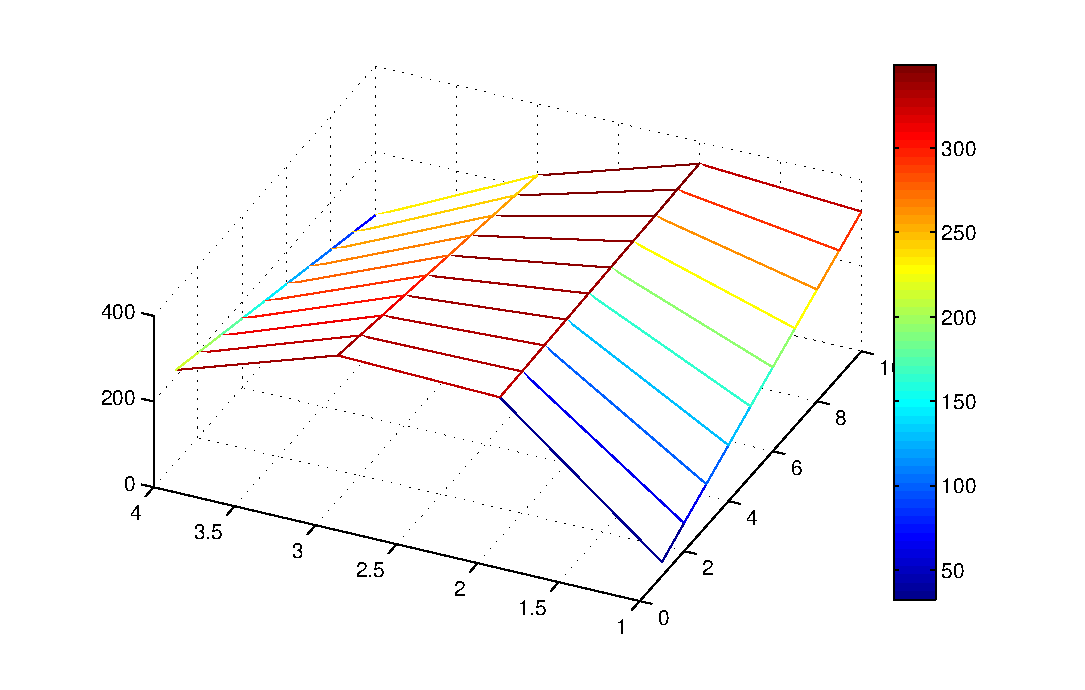
\includegraphics[scale=0.7]{innoscore.eps}}
 \caption{创新班课表分数}
 \end{figure}
 \begin{figure}[H]
 \centerline{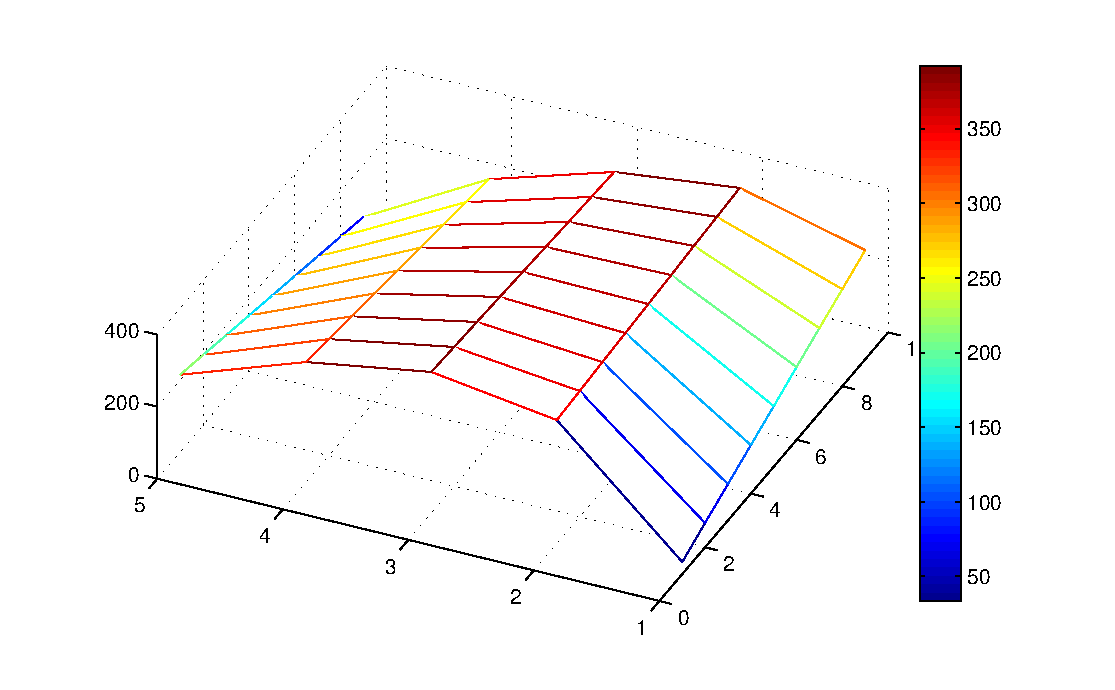
\includegraphics[scale=0.7]{normscore.eps}}
 \caption{平行班课表分数}
 \end{figure}
 通过我们对于这两张课表的打分, 我们可以发现其实现有课表的分值并不高, 所以我们将之前的打分模型, 在后文对于现有课表进行调整和优化.
 \clearpage
 \subsection{优化模型: 教师打分模型}
  我们其实可以发现没有一节课的授课成效是只和学生接受效率有关的, 同样的老师的授课效率也是至关重要的一环, 如果老师的授课效率低下, 即使学生状态再好, 学习的效果也是不高的. 所以在这个模型中我们将研究老师的授课效率, 以及学生与老师的综合效率问题.
  \subsubsection{老师的授课效率模型}
   \paragraph{变量}
   \begin{center}
   \begin{tabular}{|p{30pt}|p{250pt}|}
   \hline
   \bf\hfil 变量 & \bf\hfil 说\quad 明\\\hline
   $\matrix{P}_\text{转减}$ & 老师下节课上课状态转移矩阵 \\\hline
   $\matrix{P}_\text{转增}$ & 老师下节课不上课状态转移矩阵 \\\hline
   $\matrix{P}_\text{初}$ & 老师授课效率的初状态 \\\hline
   $\matrix{P}_\text{末}$ & 老师授课效率的末状态 \\\hline
   \end{tabular}
   \end{center}
   首先进行感性分析, 设计一份老师喜欢的课表对于提升老师的授课效率有着巨大的影响, 然而对于不同的老师, 都有着不同的喜好, 有的老师喜欢或者习惯一次性的上完一天的课, 比如上午时候连上三节课, 下午不上课, 甚至四天上完所有的课, 另一天休息, 还有的老师喜欢把课拆开来, 一节一节的上, 当然这只是老师的个人想法, 不完全做参考.\par
   接着是理性分析, 类似学生的接受效率, 老师的授课效率也是会有增减的, 我们假设老师的早晨的初始效率为满, 上完一节课后乘以一个状态的转移矩阵, 得到一个新的状态, 即:
   \begin{equation}
   \matrix{P}_\text{末}=\matrix{P}_\text{初}\times\matrix{P}_\text{转减}
   \end{equation}
   而如果下一节课老师进行休息, 那么老师的状态将会回升 (同样也是乘以一个状态转移矩阵), 即
   \begin{equation}
   \matrix{P}_\text{末}=\matrix{P}_\text{初}\times\matrix{P}_\text{转增}
   \end{equation}
   同样的下午的时候老师也会有一个午间的初始状态 (类似学生), 依据以上的分析, 我们就可以计算得出老师在一天各节课中的授课效率. 在根据之前对于老师上课喜好的调查与统计, 我们就可以对于老师的授课效率进行综合的打分.
  \clearpage
  \subsubsection{学生与老师的综合效率评定}
   \paragraph{变量与常量}
   \begin{center}
   \begin{tabular}{|p{30pt}|p{250pt}|}
   \hline
   \bf\hfil 变量 & \bf\hfil 说\quad 明\\\hline
   $Y$ & 学生学习效果 (产量)\\\hline
   $K$ & 老师的授课效率 (投入资本量)\\\hline
   $L$ & 学生的学习效率 (投入劳动力)\\\hline
   \end{tabular}\\[2mm]
   \begin{tabular}{|p{30pt}|p{250pt}|}
   \hline
   \bf\hfil 常量 & \bf\hfil 说\quad 明\\\hline
   $A$ & 学生素质 (技术水平)\\\hline
   $\alpha$ & $K$\,的产出弹性\\\hline
   $\beta$ & $L$\,的产出弹性\\\hline
   \end{tabular}
   \end{center}
   首先我们分析\,Cobb-Douglas\,生产函数\,\cite{ISBN9787040311501-2}\,与学生学习之间的联系, 在\,Cobb-Douglas\,生产函数中, 有着产量与技术水平, 投入资本量, 投入劳动力的函数关系, 而在学生的学习上面, 同样也存在着学生学习效果 (主要表现形式为考试成绩) 与学生素质, 老师的授课效率, 学生的学习效率之间的函数关系, 所以我们在这里讲两者进行类比, 产量与学生的学习效果相匹配, 技术水平与学生素质相匹配 (即初始的学生学习情况与能力), 投入资本量与老师的授课相率相匹配, 投入劳动力与学生的接受效率相匹配.
   \begin{equation}
   Y=AK^\alpha L^\beta
   \end{equation}
   再根据之前论文中所得到的结果, 我们就可以得出一节课中学生与老师的综合效率, 即一节课给学生学习带来的真正提升效果. 依次对于整张课表进行完整打分.
\clearpage
\section{打分系统吻合度分析}
 我们可以发现其实对于一个合理的打分系统, 其打分得出的分值应该是和实际情况吻合度很高的, 所以我们在这里对于打分系统进行与实际情况的吻合度分析.\par
 考虑到理科班, 创新班的分数平行班的分数存在一定的差距, 所以我们分理科班和创新班, 平行班两组进行打分系统的吻合度分析, 依此来评判我们的打分系统合理性.
 \subsection{平行班的吻合度分析}
  首先我们统计了平行班班级同学在第一学期期末考试各科的成绩, 将其与各个考试科目的重要程度相乘, 得到了总的打分分数, 即平行班分数图像的子图\,1.\par
  接着我们统计了平行班班级在三次大考试 (第一学期期中期末考试的成绩和第二学期期中考试) 中的五总总分的平均分以及三次考试的平均分, 图像见平行班分数图像的子图\,2.\par
  其次我们统计了各个班级的优良率, 见平行班分数图像的子图\,3.\par
  在平行班分数图像的子图\,4\,中显示了\,4\,个平行班的具体打分分数.\par
  \begin{figure}[H]
  \centerline{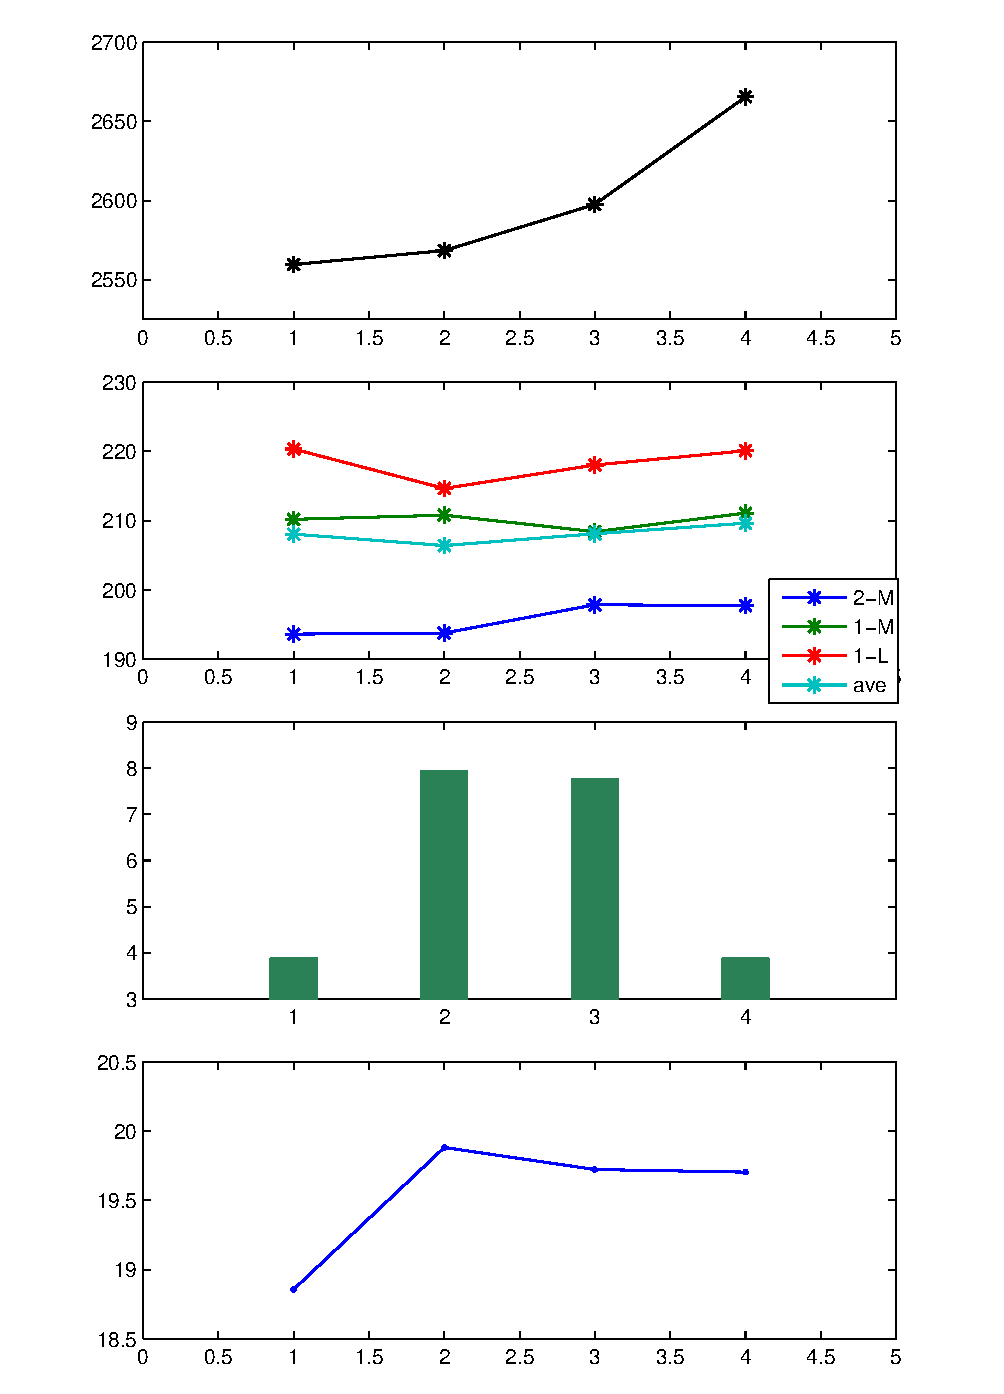
\includegraphics[scale=0.5]{result.eps}}
  \caption{平行班分数}
  \end{figure}
  然后我们基于以上数据计算得出了平行班打分系统的吻合度.
  \begin{table}[H]
  \centering
  \begin{tabular}{|c|c|c|c|c|}
  \hline
  \bf 班级 & \bf 总分 & \bf 课表分数 & \bf 吻合度 & \bf 取\,3\,班为一 \\\hline
  \bf 1 & 2559.59 & 18.855944 & 135.7444634 & 1.030666908 \\\hline
  \bf 2 & 2568.42 & 19.881084 & 129.1891327 & 0.980894253 \\\hline
  \bf 3 & 2597.6 & 19.722796 & 131.7054641 & 1 \\\hline
  \bf 4 & 2665.48 & 19.704152 & 135.2750425 & 1.027102736 \\\hline
  \end{tabular}\\[2mm]
  \begin{tabular}{|c|c|c|c|c|}
  \hline
  \bf 班级 & \bf 平均分 & \bf 课表分数 & \bf 吻合度 & \bf 取\,3\,班为一 \\\hline
  \bf 1 & 208.0566667 & 18.855944 & 11.03400958 & 1.045754541 \\\hline
  \bf 2 & 206.4066667 & 19.881084 & 10.38206301 & 0.983965933 \\\hline
  \bf 3 & 208.1 & 19.722796 & 10.55124233 & 1 \\\hline
  \bf 4 & 209.63 & 19.704152 & 10.63887449 & 1.008305388 \\\hline
  \end{tabular}\\[2mm]
  \begin{tabular}{|c|c|c|c|c|}
  \hline
  \bf 班级 & \bf 优良率 & \bf 课表分数 & \bf 吻合度 & \bf 取\,3\,班为一 \\\hline
  \bf 1 & 3.876666667 & 18.855944 & 0.205593879 & 0.523211114 \\\hline
  \bf 2 & 7.936666667 & 19.881084 & 0.399206938 & 1.015932516 \\\hline
  \bf 3 & 7.75 & 19.722796 & 0.392946315 & 1 \\\hline
  \bf 4 & 3.876666667 & 19.704152 & 0.196743644 & 0.500688356 \\\hline
  \end{tabular}
  \caption{平行班的吻合度分析}
  \end{table}
  根据以上数据我们绘制了吻合度的图像, 其中我们选取\,3\,班为基准, 根据之前的三类数据分别绘制了三张子图.
  \begin{figure}[H]
  \centerline{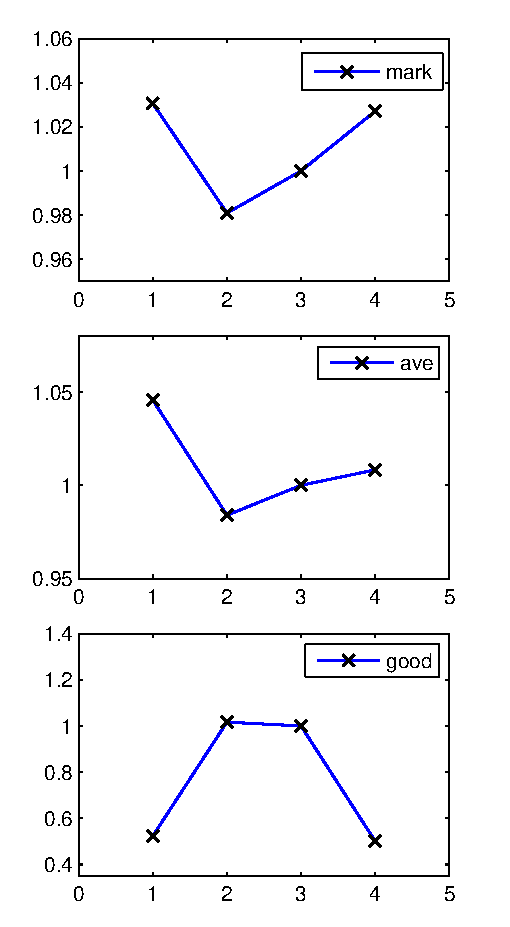
\includegraphics[scale=0.5]{coincidenorm.eps}}
  \caption{平行班的吻合度分析}
  \end{figure}
  我们可以发现在平行班的打分中吻合度还是较高的.
 \clearpage
 \subsection{理科班和创新班的吻合度分析}
  相同的, 我们根据平行班的分析方法, 分析理科班和创新班的吻合度, 得出了以下分数.
  \begin{table}[H]
  \centering
  \begin{tabular}{|c|c|c|c|c|c|}
  \hline
  \bf 班级 & \bf 总分 & \bf 课表分数 & \bf 吻合度 & \bf 取\,6\,班为一 & \bf 取\,5\,班为一 \\\hline
  \bf 5 & 2918.37 & 19.790304 & 147.4646372 & 1.005146244 & 1 \\\hline
  \bf 6 & 2887.37 & 19.680848 & 146.7096336 & 1 & 0.994880104 \\\hline
  \end{tabular}\\[2mm]
  \begin{tabular}{|c|c|c|c|c|c|}
  \hline
  \bf 班级 & \bf 总分 & \bf 课表分数 & \bf 吻合度 & \bf 取\,6\,班为一 & \bf 取\,5\,班为一 \\\hline
  \bf 5 & 232.1567 & 19.790304 & 11.73082873 & 1.000994279 & 1 \\\hline
  \bf 6 & 230.6433 & 19.680848 & 11.7191766 & 1 & 0.999006709 \\\hline
  \end{tabular}\\[2mm]
  \begin{tabular}{|c|c|c|c|c|c|}
  \hline
  \bf 班级 & \bf 总分 & \bf 课表分数 & \bf 吻合度 & \bf 取\,6\,班为一 & \bf 取\,5\,班为一 \\\hline
  \bf 5 & 23.33 & 19.790304 & 1.179028545 & 0.812190465 & 1 \\\hline
  \bf 6 & 28.57 & 19.680848 & 1.451665091 & 1 & 1.231238291 \\\hline
  \end{tabular}
  \caption{理科班和创新班的吻合度分析}
  \end{table}
  我们分别选取\,6\,班 (子图\,2) 和\,5\,班 (子图\,1) 为基准, 绘制了理科班和创新班吻合度图像.
  \begin{figure}[H]
  \centerline{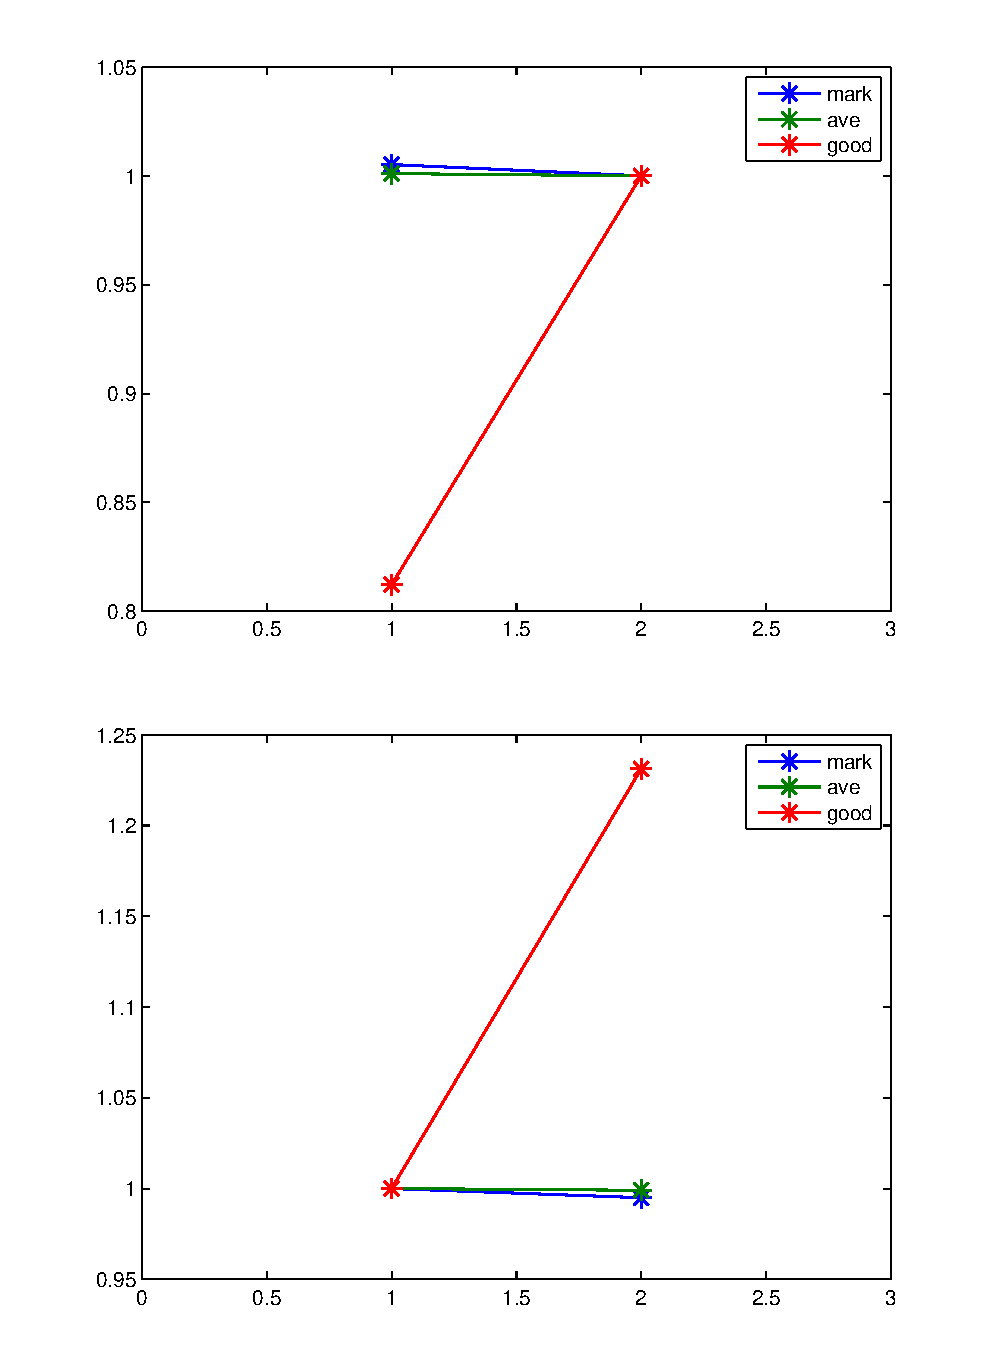
\includegraphics[scale=0.4]{coincideinno.eps}}
  \caption{理科班和创新班的吻合度分析}
  \end{figure}
  我们发现除了优良率有一定的偏差, 其余的基本没有偏差.\par
  综上我们可以发现, 我们所提出的打分系统和实际的情况吻合度还是很高的, 所以前文提出的打分系统还是比较合理的.
\clearpage
\section{课表的基本优化设计 (计算机模型)}
 根据上文的分析我们将对现有的课表进行优化.\par
 在这里我们将先进行基本的优化, 即提高整张课表的打分分值而不改变一些基本的条件.
 \subsection{算法分析}
  我们在这里使用模拟退火算法\,\cite{ISBN9787512403178}\,得到较优的课表解.\par
  {\bf 具体算法}: 我们将课表进行调整, 我们首先定义两种不同的交换方式, 一种是行交换, 一种是列交换. 接着我们通过这些交换, 比运用了模拟退火算法得出了较优课表.\par
  \begin{figure}[H]
  \centering
  \begin{tikzpicture}[thick]
  \tikzset{inoutput/.style={trapezium,trapezium left angle=60,trapezium right angle=120}}
  \def\smbwd{2cm}
  \node (start) at (0,13.5) [draw, terminal,
  minimum width=2cm,
  minimum height=0.5cm] {开始};
  \node (input) at (0,12.5) [draw, inoutput,
  minimum width=\smbwd,
  minimum height=0.5cm] {输入课表};
  \node (loop1) at (0,11) [draw, decision,
  minimum width=\smbwd,
  minimum height=0.5cm,
  inner sep=-4pt] {第一重循环};
  \node (loop2) at (0,9) [draw, decision,
  minimum width=\smbwd,
  minimum height=0.5cm,
  inner sep=-4pt] {第二重循环};
  \node (randomdecision) at (0,7) [draw, decision,
  minimum width=\smbwd,
  minimum height=0.5cm,
  inner sep=-4pt] {随机判断};
  \node (rs) at (-2,6) [draw, process,
  minimum width=\smbwd,
  minimum height=0.5cm] {行交换};
  \node (cs) at (2,6) [draw, process,
  minimum width=\smbwd,
  minimum height=0.5cm] {列交换};
  \node (score) at (0,4) [draw, process,
  minimum width=\smbwd,
  minimum height=0.5cm] {打分};
  \node (accept) at (0,3) [draw, process,
  minimum width=\smbwd,
  minimum height=0.5cm] {接受与否};
  \node (output) at (0,1) [draw, inoutput,
  minimum width=\smbwd,
  minimum height=0.5cm] {输出课表};
  \node (end) at (0,0) [draw, terminal,
  minimum width=\smbwd,
  minimum height=0.5cm] {结束};
  \coordinate (prs) at (-2,7);
  \coordinate (pcs) at (2,7);
  \coordinate (prsend) at (-2,5);
  \coordinate (pcsend) at (2,5);
  \coordinate (pend) at (0,5);
  \coordinate (p1loop) at (-3.5,3);
  \coordinate (p2loop) at (-3.5,10);
  \coordinate (p3loop) at (0,10);
  \coordinate (p1loop2) at (3.5,9);
  \coordinate (p2loop2) at (3.5,2.2);
  \coordinate (p3loop2) at (-4,2.2);
  \coordinate (p4loop2) at (-4,12);
  \coordinate (p5loop2) at (0,12);
  \coordinate (p1loop1) at (4,11);
  \coordinate (p2loop1) at (4,1.6);
  \coordinate (p3loop1) at (0,1.6);
  \draw[->] (start) -- (input);
  \draw[->] (input) -- (loop1);
  \draw[->] (loop1) -- node[right]{第一重循环未结束} (loop2);
  \draw[->] (loop2) -- node[right]{第二重循环未结束} (randomdecision);
  \draw[->] (randomdecision) -- node[above]{Y} (prs) -- (rs);
  \draw[->] (randomdecision) -- node[above]{N} (pcs) -- (cs);
  \draw[->] (rs) -- (prsend) -- (pend) -- (score);
  \draw[->] (cs) -- (pcsend) -- (pend) -- (score);
  \draw[->] (score) -- (accept);
  \draw[->] (accept) -- (p1loop) -- (p2loop) -- (p3loop);
  \draw[->] (loop2) -- node[above]{第二重循环结束} (p1loop2) -- (p2loop2) -- (p3loop2) -- (p4loop2) -- (p5loop2);
  \draw[->] (loop1) -- node[above]{第一重循环结束} (p1loop1) -- (p2loop1) -- (p3loop1) -- (output);
  \draw[->] (output) -- (end);
  \end{tikzpicture}
  \caption{算法流程图}
  \end{figure}
 \clearpage
 \subsection{结果分析}
  通过之前的算法, 我们编写程序得到了优化的课表评分. 首先是理科班及平行班, 这两类班级的坑成数目设置是一致的, 所以我们将其一起考虑, 进行优化. 接着是创新班, 由于其特殊的课程安排, 我们将其单独进行了课表的优化, 由于其周三下午多了四节特需课的缘故, 所以少了三节课列入打分范围, 故分数整体偏低. 各班课表优化得到的具体分数见图像.
  \begin{figure}[H]
  \centerline{\begin{overpic}[scale=0.4]{goodlesson.eps}
  \put(49,1){\colorbox{white}{课程}}
  \put(5,29){\rotatebox{90}{\colorbox{white}{成绩}}}
  \put(48,57.8){\colorbox{white}{\qquad\quad}}
  \end{overpic}}
  \caption{理科班及平行班课表最优成绩}
  \end{figure}
  \begin{figure}[H]
  \centerline{\begin{overpic}[scale=0.4]{goodmark.eps}
  \put(49,1){\colorbox{white}{课程}}
  \put(5,29){\rotatebox{90}{\colorbox{white}{成绩}}}
  \put(48,57.8){\colorbox{white}{\qquad\quad}}
  \end{overpic}}
  \caption{创新班课表最优成绩}
  \end{figure}
  这里我们可以发现, 我们计算得出的只是单个课表在满足基本条件的情况下得出的局部近似最优解, 即没有考虑整个年级下的冲突问题. 我们将在\,6.4\,中整年级课表的安排中进行具体分析.
 \clearpage
 \subsection{敏感度分析}
  我们可以很明显地发现在之前的程序中有很多的参数是直接得到的, 没有写出直接的理由. 我们在这里着重对于状态转移矩阵进行敏感度分析.\par
  我们将矩阵先量化, 这里我们例举了重要程度为\,3\,的课程的二阶状态转移矩阵.\par
  \begin{equation}
  \matrix{Q}=
  \begin{bmatrix}
  1-0.3q_{12} & 0.3q_{12} \\
  1-0.3q_{22} & 0.3q_{22}
  \end{bmatrix}
  \end{equation}
  我们发现实际二阶状态转移矩阵这里只有两个变量, 另一个是独立的重要程度变量, 在之前的敏感度分析中我们已经发现其敏感性并不强, 所以这里不再一并讨论, 只对这两个参数进行分析. 我们得到了以下结果.
  \begin{figure}[H]
  \centerline{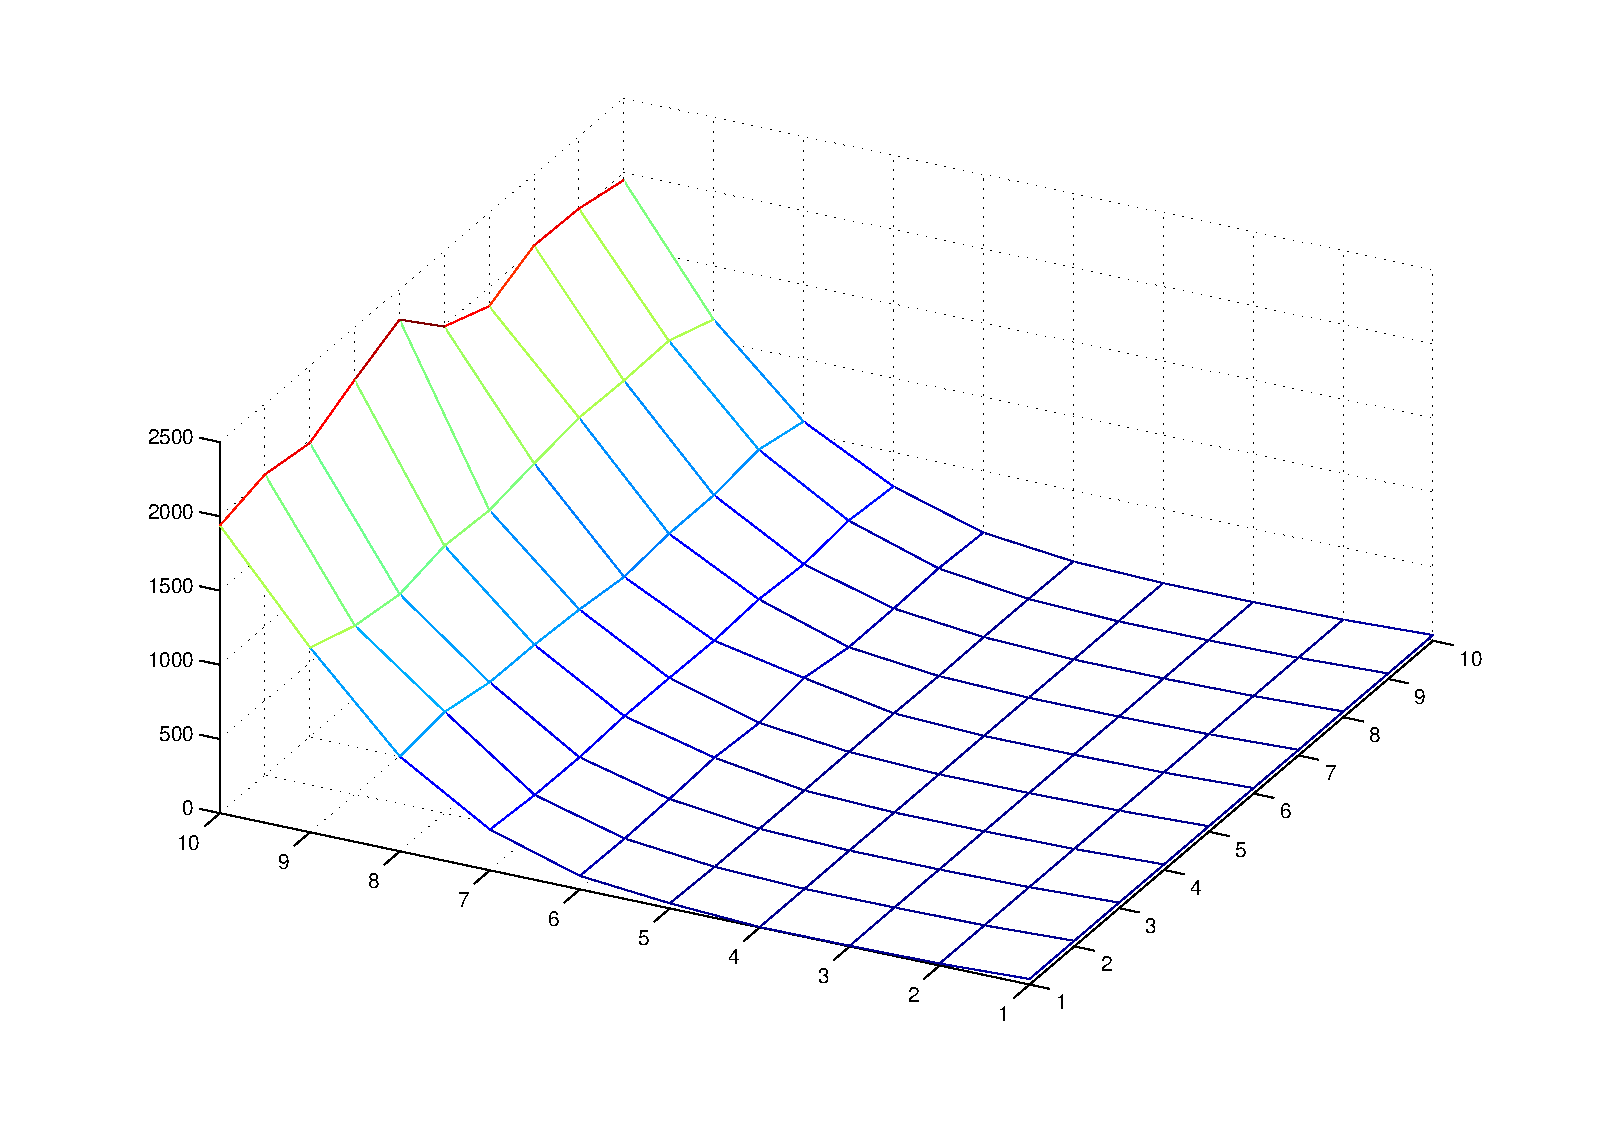
\includegraphics[scale=0.5]{inno2.eps}}
  \caption{创新班二阶状态转移矩阵的敏感度分析}
  \end{figure}
  我们很容易就会发现打分值对于状态转移矩阵很敏感, 所以我们有选取了总区间中的敏感度较弱的部分进行分析.
  \begin{figure}[H]
  \centerline{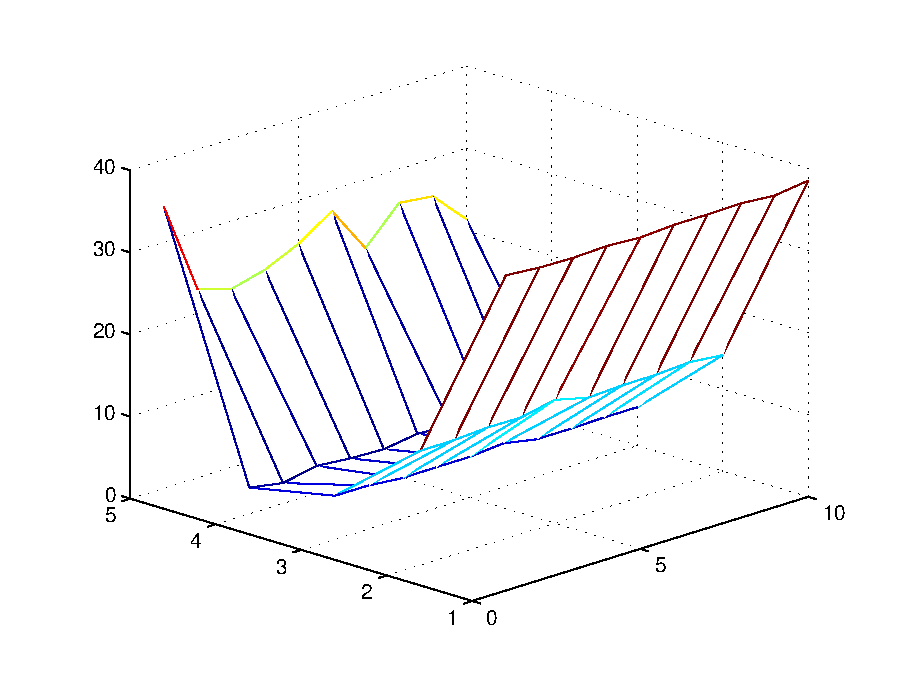
\includegraphics[scale=0.7]{inno2part.eps}}
  \caption{创新班二阶状态转移矩阵的敏感度分析 (局部图)}
  \end{figure}
  根据上一张图像我们就基本确定了\,$q_{12}$, $q_{22}$\,的值, 均在区间\,$[3,4]$\,最为合适, 即敏感度较弱.\par
  同理, 我们基于二阶状态转移矩阵的分析结果, 推出了三阶状态转移矩阵的情况.
  \begin{equation}
  \matrix{P}=
  \begin{bmatrix}
  1-0.3p_{12}-0.3p_{13} & 0.3p_{12} & 0.3p_{13} \\
  1-0.3p_{22}-0.3p_{23} & 0.3p_{22} & 0.3p_{23} \\
  0 & 0 & 1
  \end{bmatrix}
  \end{equation}
  注意到左上角的\,$2\times2$\,矩阵中内容和二阶状态转移矩阵内容意义相同, 所以借用之前的二阶状态转移矩阵的敏感度分析结果, 取敏感度较弱部分的数据作为结果, 将\,$p_{12}$, $p_{22}$\,定为常量. 然后就将问题转化为两个变量的敏感度分析. 我们得到了以下结果.
  \begin{figure}[H]
  \centerline{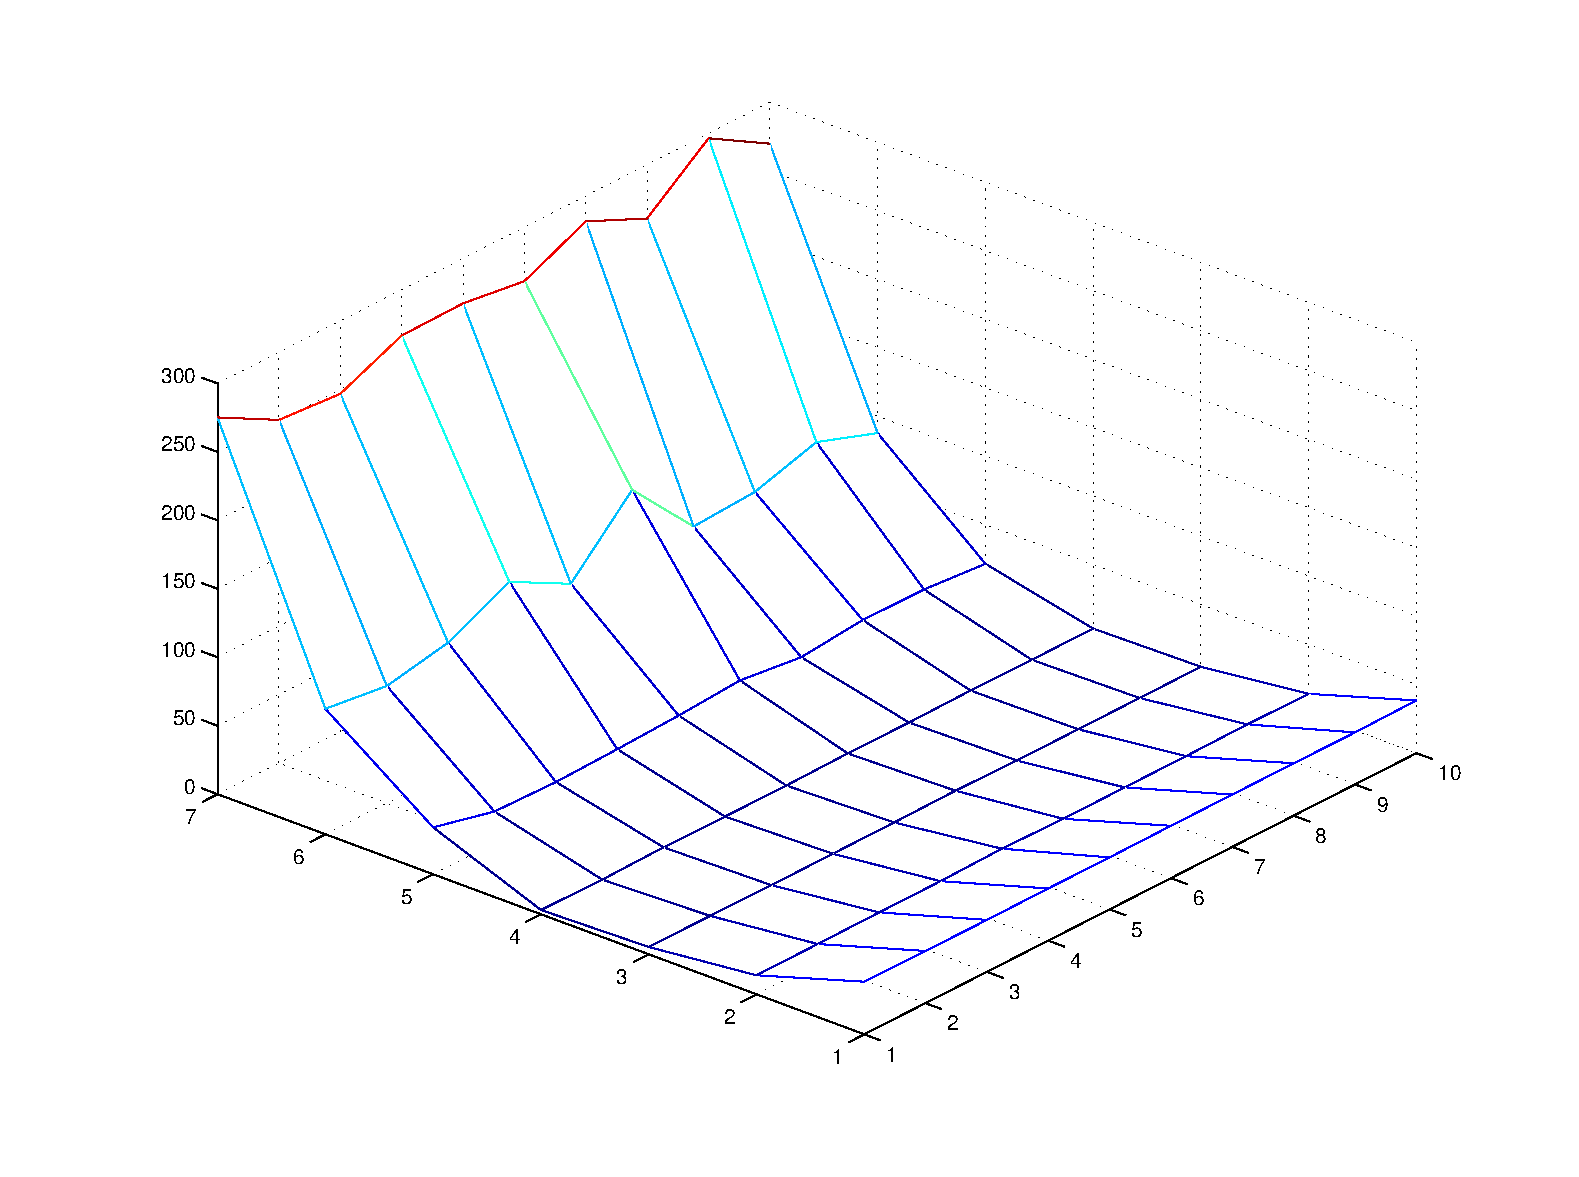
\includegraphics[scale=0.5]{inno3.eps}}
  \caption{创新班三阶状态转移矩阵的敏感度分析}
  \end{figure}
  同样的, 介于其敏感度较大我们选取总区间中的敏感度较弱的部分进行分析.
  \begin{figure}[H]
  \centerline{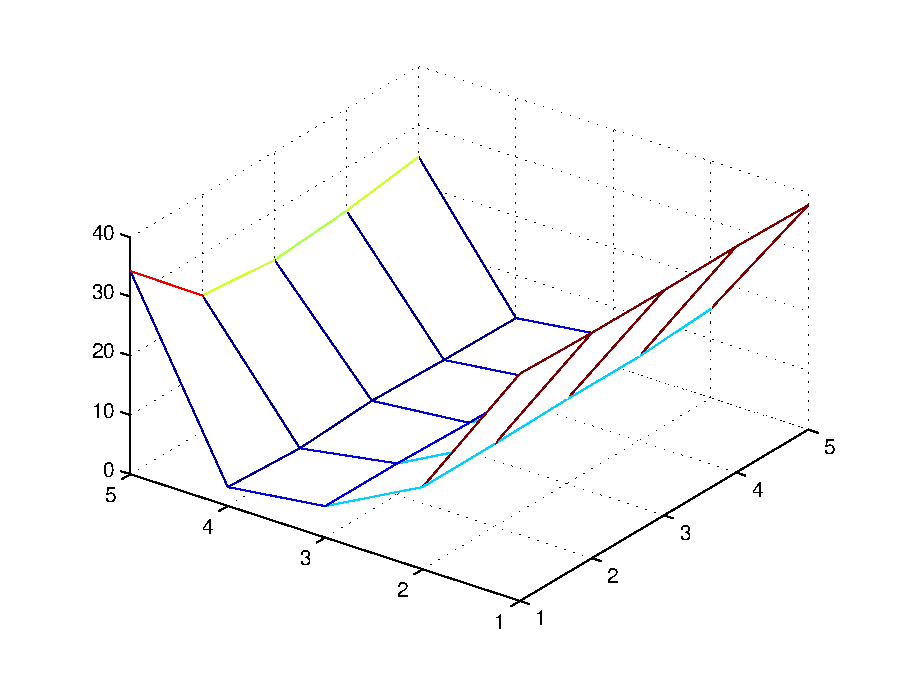
\includegraphics[scale=0.7]{inno3part.eps}}
  \caption{创新班三阶状态转移矩阵的敏感度分析 (局部图)}
  \end{figure}
  依此, 我们确定了\,$p_{22}$, $p_{23}$\,的范围, 基本在\,$[3,4]$\,和\,$[2,5]$\,之间.\par
  同理我们对于理科班及平行班也进行了相同的分析, 这里就直接列举三阶状态转移矩阵敏感度分析的图像.
  \begin{figure}[H]
  \centerline{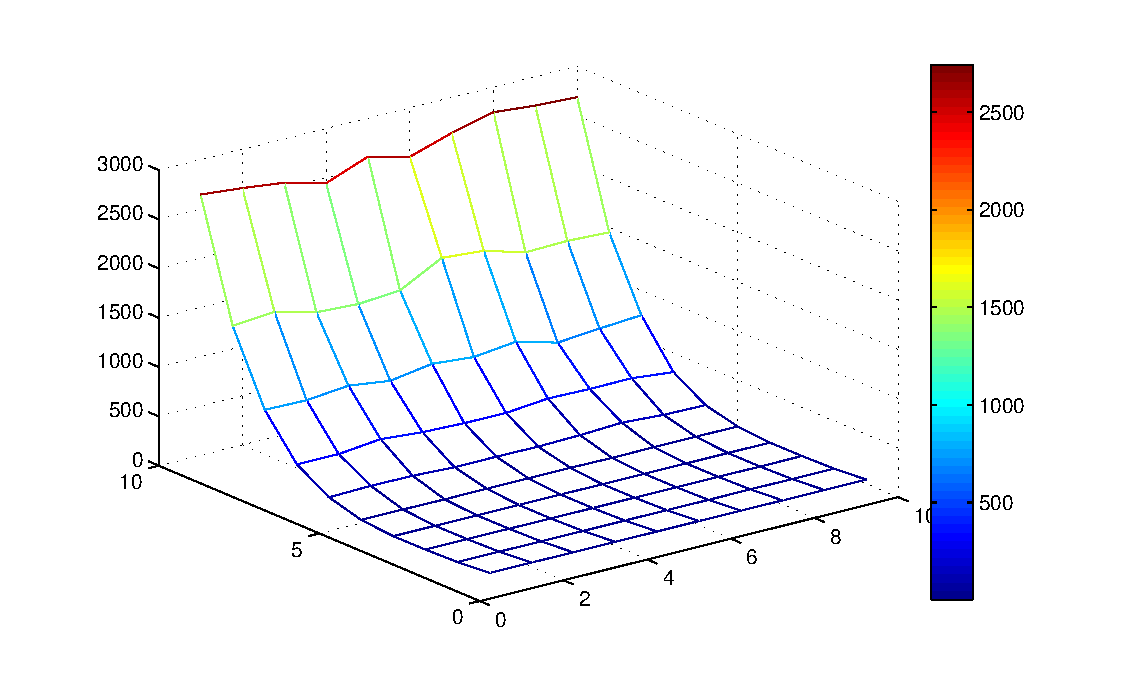
\includegraphics[scale=0.7]{norm3.eps}}
  \caption{理科班及平行班三阶状态转移矩阵的敏感度分析}
  \end{figure}
  \begin{figure}[H]
  \centerline{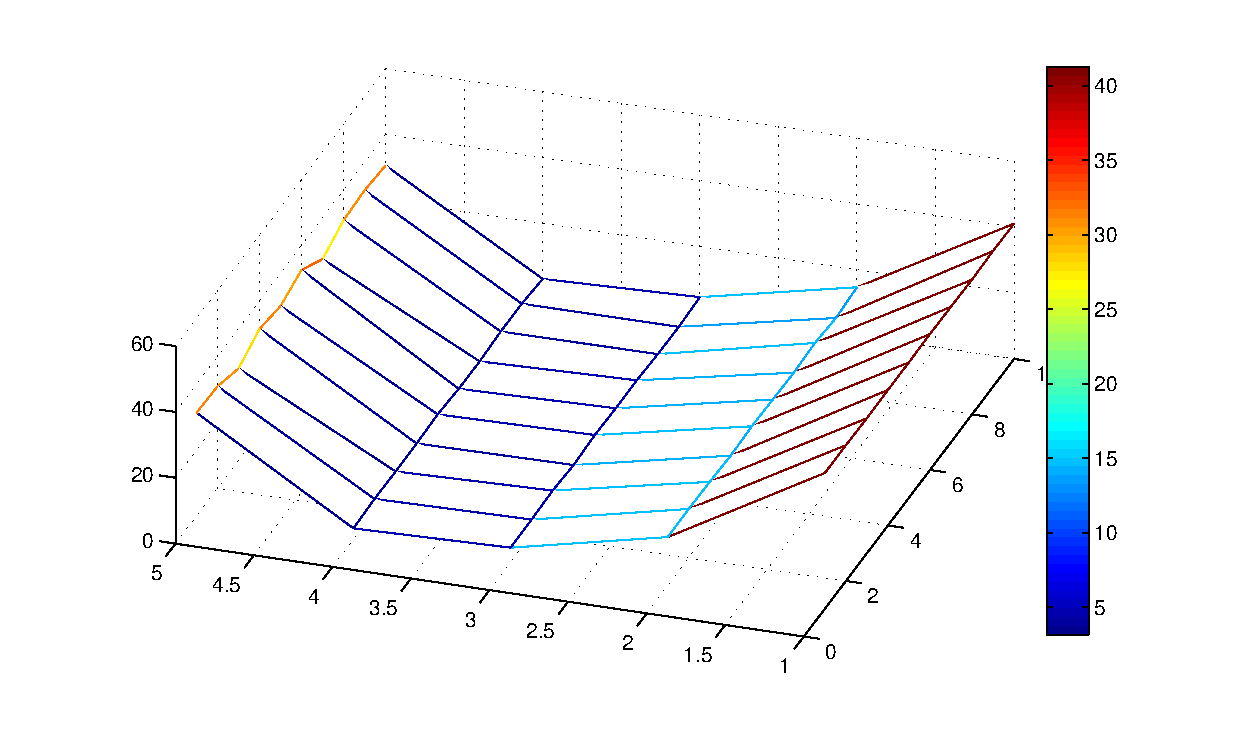
\includegraphics[scale=0.7]{norm3part.eps}}
  \caption{理科班及平行班三阶状态转移矩阵的敏感度分析 (局部图)}
  \end{figure}
 \clearpage
 \subsection{最优课表输出}
  根据之前我们已经得到的最优课表, 我们进行整合, 首先有几个基本的条件:\par
  1. 有两节语文的连堂课.\par
  2. 有两节信息科技的连堂课.\par
  3. 老师不能同时上两个班的课.\par
  \begin{table}[H]
  \centering
  \begin{tabular}{|l|p{50pt}p{50pt}p{50pt}p{50pt}|}
  \hline
  语文 & 1 5 & 2 6 & 3 4 & \\\hline
  英语 & 1 2 & 3 & 4 6 & 5 \\\hline
  数学 & 1 2 & 3 5 & 4 & 6 \\\hline
  物理 & 1 2 3 & 4 5 6 & & \\\hline
  化学 & 1 2 & 3 4 5 & 6 & \\\hline
  政治 & 1 2 3 4 5 6 & & & \\\hline
  历史 & 1 3 5 & 2 4 6 & & \\\hline
  信息 & 1 2 3 4 & 5 6 & & \\\hline
  地理 & 1 2 & 3 4 5 6 & & \\\hline
  音乐 & 1 3 5 & 2 4 6 & & \\\hline
  体育 & 1 2 3 4 5 6 & & & \\\hline
  研究 & 1 2 3 4 5 6 & & & \\\hline
  \end{tabular}
  \caption{同一老师上课的班级}
  \end{table}
  4. 体育课必须有两个班一起上.\par
  5. 活动课必须有三个班一起上.\par
  通过以上的条件和之前的结果, 我们调整得出了一份高一整个年级的较优课表. 具体课表见下.
  \clearpage
  \subsubsection{高一(1)班}
   \begin{tabular}{|c|c|c|c|c|c|}
   \hline
   & \bf 星期一 & \bf 星期二 & \bf 星期三 & \bf 星期四 & \bf 星期五 \\\hline
   \bf 1 & 英语 & 语文 & 数学 & 英语 & 数学 \\\hline
   \bf 2 & 物理 & 语文 & 历史 & 数学 & 物理 \\\hline
   \bf 3 & 研究 & 音乐 & 信息 & 化学 & 地理 \\\hline
   \bf 4 & 化学 & 体育 & 信息 & 语文 & 英语 \\\hline
   \bf 5 & 语文 & 数学 & 物理 & 政治 & 语文 \\\hline
   \bf 6 & 数学 & 英语 & 英语 & 历史 & 政治 \\\hline
   \bf 7 & 活动 & 地理 & 化学 & 体育 & 班会 \\\hline
   \bf 8 & 拓展 & TFT  & 特需 & 地理 & 社团 \\\hline
   \end{tabular}
  \subsubsection{高一(2)班}
   \begin{tabular}{|c|c|c|c|c|c|}
   \hline
   & \bf 星期一 & \bf 星期二 & \bf 星期三 & \bf 星期四 & \bf 星期五 \\\hline
   \bf 1 & 数学 & 物理 & 语文 & 数学 & 物理 \\\hline
   \bf 2 & 英语 & 政治 & 语文 & 化学 & 数学 \\\hline
   \bf 3 & 地理 & 化学 & 化学 & 信息 & 历史 \\\hline
   \bf 4 & 政治 & 体育 & 英语 & 信息 & 地理 \\\hline
   \bf 5 & 语文 & 英语 & 数学 & 语文 & 研究 \\\hline
   \bf 6 & 物理 & 语文 & 音乐 & 英语 & 英语 \\\hline
   \bf 7 & 活动 & 数学 & 地理 & 体育 & 班会 \\\hline
   \bf 8 & 拓展 & TFT  & 特需 & 历史 & 社团 \\\hline
   \end{tabular}
  \subsubsection{高一(3)班}
   \begin{tabular}{|c|c|c|c|c|c|}
   \hline
   & \bf 星期一 & \bf 星期二 & \bf 星期三 & \bf 星期四 & \bf 星期五 \\\hline
   \bf 1 & 数学 & 英语 & 语文 & 数学 & 化学 \\\hline
   \bf 2 & 地理 & 体育 & 语文 & 英语 & 数学 \\\hline
   \bf 3 & 英语 & 政治 & 英语 & 化学 & 语文 \\\hline
   \bf 4 & 语文 & 历史 & 数学 & 研究 & 物理 \\\hline
   \bf 5 & 信息 & 数学 & 地理 & 历史 & 音乐 \\\hline
   \bf 6 & 信息 & 物理 & 物理 & 地理 & 英语 \\\hline
   \bf 7 & 活动 & 语文 & 化学 & 体育 & 班会 \\\hline
   \bf 8 & 拓展 & TFT  & 特需 & 政治 & 社团 \\\hline
   \end{tabular}
  \clearpage
  \subsubsection{高一(4)班}
   \begin{tabular}{|c|c|c|c|c|c|}
   \hline
   & \bf 星期一 & \bf 星期二 & \bf 星期三 & \bf 星期四 & \bf 星期五 \\\hline
   \bf 1 & 数学 & 数学 & 英语 & 数学 & 语文 \\\hline
   \bf 2 & 物理 & 体育 & 数学 & 语文 & 语文 \\\hline
   \bf 3 & 政治 & 语文 & 政治 & 英语 & 数学 \\\hline
   \bf 4 & 活动 & 英语 & 音乐 & 历史 & 物理 \\\hline
   \bf 5 & 英语 & 地理 & 信息 & 研究 & 英语 \\\hline
   \bf 6 & 语文 & 物理 & 信息 & 历史 & 化学 \\\hline
   \bf 7 & 化学 & 化学 & 地理 & 体育 & 班会 \\\hline
   \bf 8 & 拓展 & TFT  & 特需 & 地理 & 社团 \\\hline
   \end{tabular}
  \subsubsection{高一(5)班 (理科班)}
   \begin{tabular}{|c|c|c|c|c|c|}
   \hline
   & \bf 星期一 & \bf 星期二 & \bf 星期三 & \bf 星期四 & \bf 星期五 \\\hline
   \bf 1 & 英语 & 数学 & 语文 & 英语 & 数学 \\\hline
   \bf 2 & 数学 & 英语 & 语文 & 数学 & 语文 \\\hline
   \bf 3 & 化学 & 历史 & 英语 & 体育 & 地理 \\\hline
   \bf 4 & 活动 & 体育 & 政治 & 地理 & 政治 \\\hline
   \bf 5 & 物理 & 信息 & 化学 & 历史 & 化学 \\\hline
   \bf 6 & 语文 & 信息 & 物理 & 音乐 & 英语 \\\hline
   \bf 7 & 研究 & 地理 & 数学 & 语文 & 班会 \\\hline
   \bf 8 & 拓展 & TFT  & 特需 & 物理 & 社团 \\\hline
   \end{tabular}
  \subsubsection{高一(6)班 (创新班)}
   \begin{tabular}{|c|c|c|c|c|c|}
   \hline
   & \bf 星期一 & \bf 星期二 & \bf 星期三 & \bf 星期四 & \bf 星期五 \\\hline
   \bf 1 & 语文 & 数学 & 数学 & 数学 & 地理 \\\hline
   \bf 2 & 语文 & 语文 & 英语 & 物理 & 英语 \\\hline
   \bf 3 & 地理 & 研究 & 历史 & 体育 & 信息 \\\hline
   \bf 4 & 活动 & 体育 & 物理 & 政治 & 信息 \\\hline
   \bf 5 & 数学 & 化学 & 特需 & 英语 & 政治 \\\hline
   \bf 6 & 物理 & 地理 & 特需 & 音乐 & 化学 \\\hline
   \bf 7 & 化学 & 英语 & 特需 & 历史 & 班会 \\\hline
   \bf 8 & 拓展 & TFT  & 特需 & 语文 & 社团 \\\hline
   \end{tabular}
 \clearpage
 \subsection{新课表打分}
  \subsubsection{基础打分}
   这是最基础的打分及其结果, 我们同时也对课表的优化率进行了分析.
   \begin{table}[H]
   \centering
   \begin{tabular}{|c|c|c|c|}
   \hline
   \bf 班级 & \bf 原始分数 & \bf 优化分数 & \bf 优化率 (\%) \\\hline
   \bf 1 & 13.903968 & 13.668048 & 1.726069443 \\\hline
   \bf 2 & 15.408372 & 15.115584 & 1.936994297 \\\hline
   \bf 3 & 15.1473032 & 15.012984 & 0.894686892 \\\hline
   \bf 4 & 15.209312 & 14.328 & 6.150977108 \\\hline
   \bf 5 & 15.191376 & 15.139416 & 0.343210068 \\\hline
   \bf 6 & 15.245984 & 14.832012 & 2.791071097 \\\hline
   \end{tabular}
   \caption{基础打分. 平均优化率: \textbf{2.307168151\%}.}
   \end{table}
   \begin{figure}[H]
   \centerline{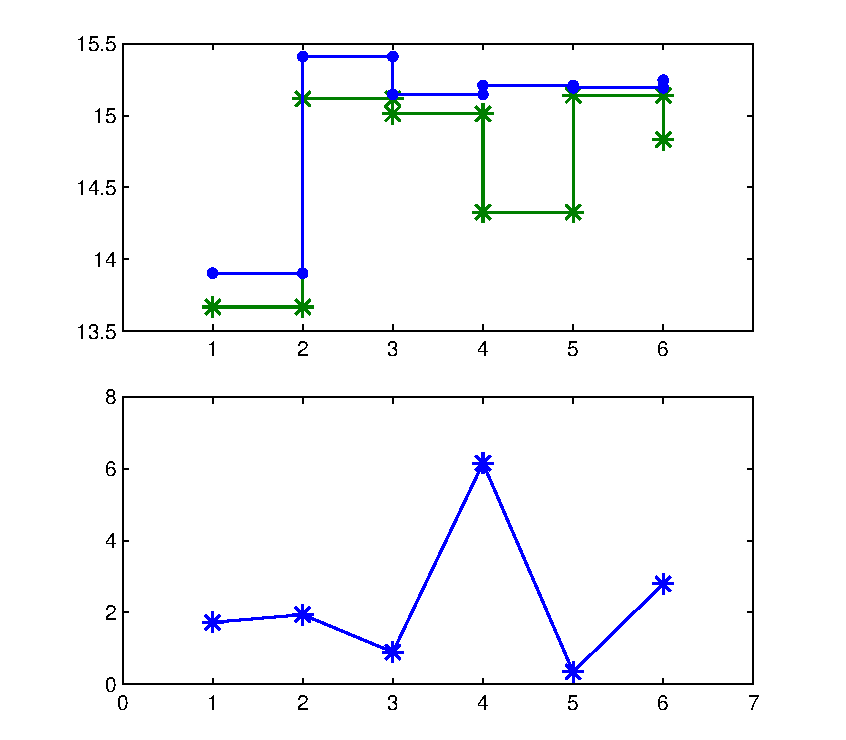
\includegraphics[scale=0.8]{mark1.eps}}
   \caption{基础打分. 上图为前后分数对比, 下图为优化率.}
   \end{figure}
   \clearpage
  \subsubsection{加入会考科目打分}
   这里我们加入了会考科目的重要程度增幅, 重新进行了打分, 并对课表的优化率进行了分析.
   \begin{table}[H]
   \centering
   \begin{tabular}{|c|c|c|c|}
   \hline
   \bf 班级 & \bf 原始分数 & \bf 优化分数 & \bf 优化率 (\%) \\\hline
   \bf 1 & 18.97016 & 18.855944 & 0.605729419 \\\hline
   \bf 2 & 20.999264 & 19.881084 & 5.624341208 \\\hline
   \bf 3 & 20.892656 & 19.722796 & 5.931511942 \\\hline
   \bf 4 & 20.462104 & 19.704152 & 3.846661353 \\\hline
   \bf 5 & 20.1849832 & 19.790304 & 1.994305898 \\\hline
   \bf 6 & 21.020516 & 19.680848 & 6.806962789 \\\hline
   \end{tabular}
   \caption{加入会考科目打分. 平均优化率: \textbf{4.134918768\%}.}
   \end{table}
   \begin{figure}[H]
   \centerline{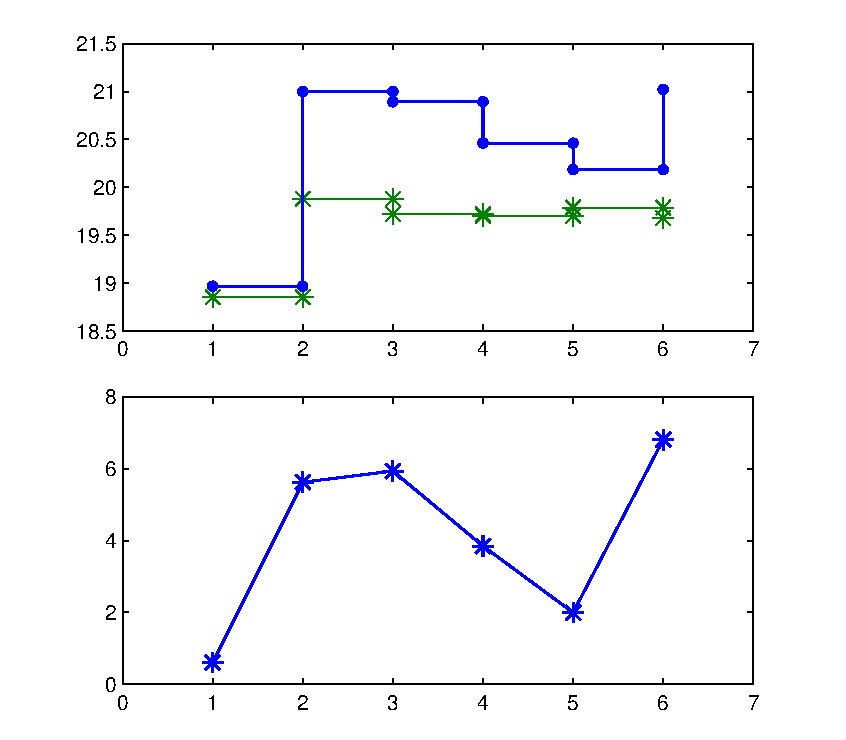
\includegraphics[scale=0.8]{mark2.eps}}
   \caption{加入会考科目打分. 上图为前后分数对比, 下图为优化率.}
   \end{figure}
  \clearpage
  \subsubsection{8\,节课打分}
   这里我们选用了敏感度分析的结论, 并加入了其他优化模型的打分, 得出了一个课表的\hyperlink{program}{\textbf{完整打分}}, 并对课表的优化率进行了分析.
   \begin{table}[H]
   \centering
   \begin{tabular}{|c|c|c|c|}
   \hline
   \bf 班级 & \bf 原始分数 & \bf 优化分数 & \bf 优化率 (\%) \\\hline
   \bf 1 & 65.30172 & 59.37332 & 9.984956206 \\\hline
   \bf 2 & 64.08168 & 57.74784 & 10.96809855 \\\hline
   \bf 3 & 60.33792 & 58.71016 & 2.772535452 \\\hline
   \bf 4 & 62.82264 & 62.194548 & 1.009882731 \\\hline
   \bf 5 & 63.48474 & 57.85312 & 9.734341035 \\\hline
   \bf 6 & 58.72536 & 57.42696 & 2.260958964 \\\hline
   \end{tabular}
   \caption{8\,节课打分. 平均优化率: \textbf{6.12179549\%}.}
   \end{table}
   \begin{figure}[H]
   \centerline{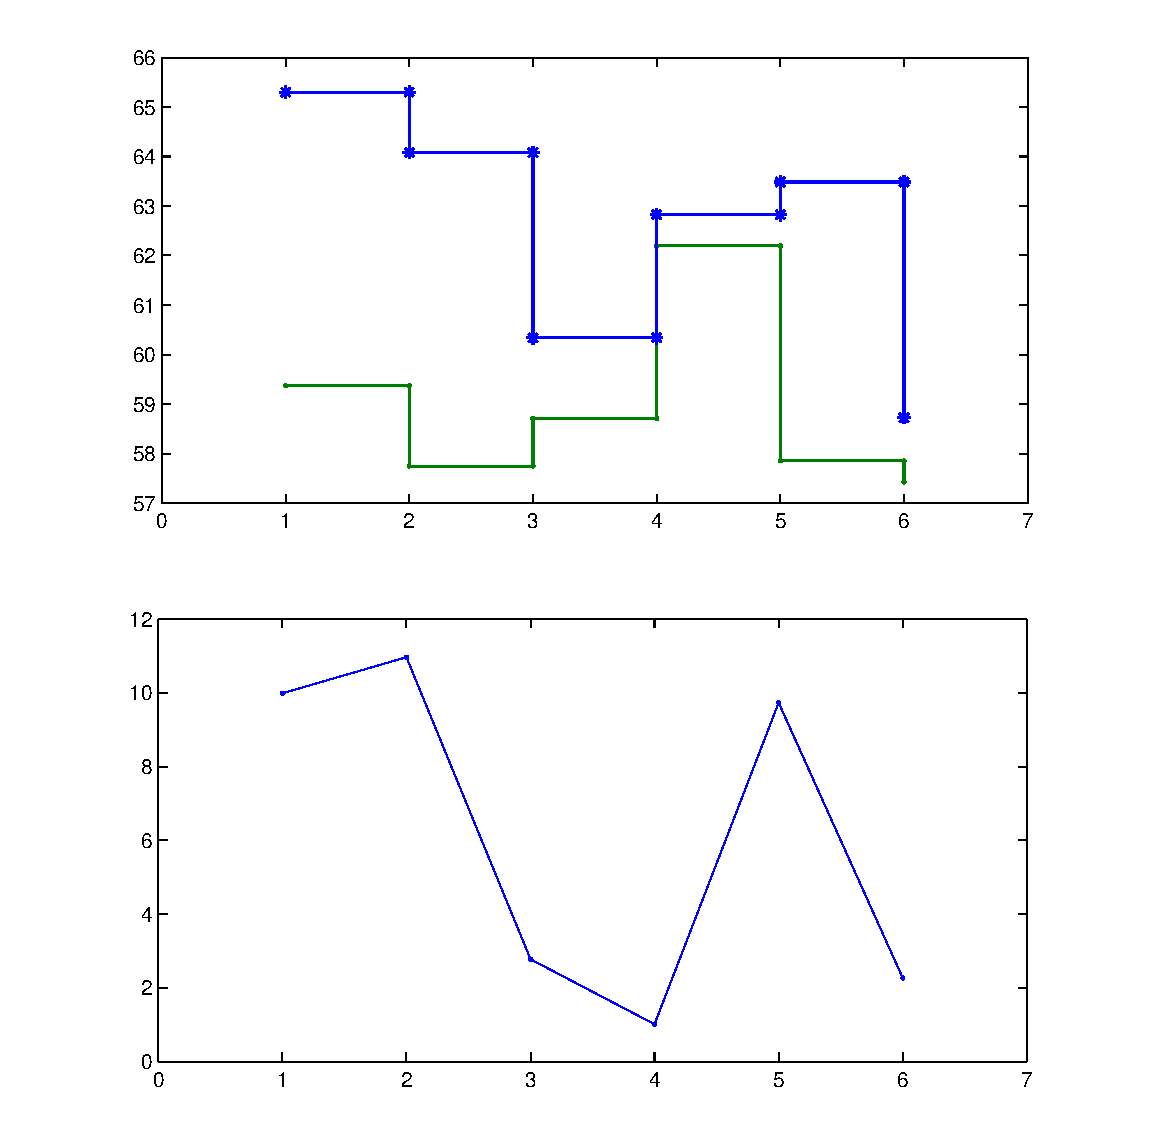
\includegraphics[scale=0.7]{8lessons.eps}}
   \caption{8\,节课打分. 上图为前后分数对比, 下图为优化率.}
   \end{figure}
\clearpage
\section{高考改制后的课表优化}
 由于政策还未公布, 所以此部分论文暂时保留.
\clearpage
\section{课时调整的课表优化 (一天\,9\,节课的调整)}
 \subsection{最优课表输出}
  我们在这里对于整个课程设置进行了调整, 我们将一天的课程调整为\,9\,节课 (去掉了早自修), 上午\,5\,节, 下午\,4\,节, 具体安排如下.
  \begin{table}[H]
  \centering
  \begin{tabular}{|l|l|}
  \hline
  \bf 时间 & \bf 课程安排 \\\hline
  7:40--8:20 & 第\,1\,节课 \\\hline
  8:30--9:10 & 第\,2\,节课 \\\hline
  \bf 9:10--9:45 & \bf 早操 \\\hline
  9:45--10:25 & 第\,3\,节课 \\\hline
  10:35--11:15 & 第\,4\,节课 \\\hline
  11:25--12:05 & 第\,5\,节课 \\\hline
  \bf 12:05--13:30 & \bf 午休 \\\hline
  13:20--14:00 & 第\,6\,节课 \\\hline
  14:10--14:50 & 第\,7\,节课 \\\hline
  \bf 14:50--15:10 & \bf 大休息 \\\hline
  15:10--15:50 & 第\,8\,节课 \\\hline
  16:00--16:40 & 第\,9\,节课 \\\hline
  \end{tabular}
  \caption{9\,节课课程安排时间表}
  \end{table}
  之前我们分析了\,8\,节课情况下的优化, 不难看出优化率并不是非常高, 无法完全达到我们课表改革的目的. 9\,节课的模式大体上将每天\,20\,分钟的早自修与最后一节\,60\,分钟的课时合并为两节\,40\,分钟的课时, 通过增加自修课, 提高学生午后学习效率, 使学生、学校双方面受益.\par
  1. 学生通过这样的\,9\,节课模式, 多出了自修课、拓展课与特需课, 从而节省了现在许多同学中午用来参与活动的时间, 中午更好的放松休息能大大提高同学们午后的学习效率.\par
  2. 学校通过这种模式节省了教师授课的部分开支, 解决了部分老师早自修与\,60\,分钟的课程安排不合理的问题; 同时学生学习效率的提高对学校总体成绩会有显著影响.\par
  而余下的课时我们将用于自修课 (每个班级增加了\,53\,分钟的自主学习时间), 这里我们对于自修课的状态转移矩阵进行定义, 我们假设同学们积极利用自修课时间, 建状态调至最佳, 这时下一节课的初始状态矩阵就转为:
  \begin{equation}
  \matrix{C}_3=
  \begin{bmatrix}
  1 & 0 & 0 \\
  1 & 0 & 0 \\
  1 & 0 & 0
  \end{bmatrix}
  \end{equation}
  由此我们编写了程序, 进行了\,9\,节课课表的优化与调整, 并得到了下面的课表.
  \clearpage
  \subsubsection{高一(1)班}
   \begin{tabular}{|c|c|c|c|c|c|}
   \hline
   & \bf 星期一 & \bf 星期二 & \bf 星期三 & \bf 星期四 & \bf 星期五 \\\hline
   \bf 1 & 英语 & 语文 & 数学 & 英语 & 数学 \\\hline
   \bf 2 & 物理 & 语文 & 历史 & 自修 & 物理 \\\hline
   \bf 3 & 自修 & 音乐 & 信息 & 数学 & 地理 \\\hline
   \bf 4 & 化学 & 体育 & 信息 & 化学 & 英语 \\\hline
   \bf 5 & 语文 & 数学 & 物理 & 语文 & 语文 \\\hline
   \bf 6 & 数学 & 英语 & 英语 & 政治 & 政治 \\\hline
   \bf 7 & 活动 & 地理 & 化学 & 历史 & 班会 \\\hline
   \bf 8 & TFT  & 研究 & 特需 & 体育 & 社团 \\\hline
   \bf 9 & 拓展 & 拓展 & 特需 & 地理 & 社团 \\\hline
   \end{tabular}
  \subsubsection{高一(2)班}
   \begin{tabular}{|c|c|c|c|c|c|}
   \hline
   & \bf 星期一 & \bf 星期二 & \bf 星期三 & \bf 星期四 & \bf 星期五 \\\hline
   \bf 1 & 数学 & 物理 & 语文 & 数学 & 物理 \\\hline
   \bf 2 & 英语 & 政治 & 语文 & 自修 & 数学 \\\hline
   \bf 3 & 地理 & 化学 & 自修 & 化学 & 历史 \\\hline
   \bf 4 & 政治 & 体育 & 化学 & 信息 & 地理 \\\hline
   \bf 5 & 语文 & 英语 & 英语 & 信息 & 研究 \\\hline
   \bf 6 & 物理 & 语文 & 数学 & 语文 & 英语 \\\hline
   \bf 7 & 活动 & 数学 & 地理 & 英语 & 班会 \\\hline
   \bf 8 & TFT  & 音乐 & 特需 & 体育 & 社团 \\\hline
   \bf 9 & 拓展 & 拓展 & 特需 & 历史 & 社团 \\\hline
   \end{tabular}
  \subsubsection{高一(3)班}
   \begin{tabular}{|c|c|c|c|c|c|}
   \hline
   & \bf 星期一 & \bf 星期二 & \bf 星期三 & \bf 星期四 & \bf 星期五 \\\hline
   \bf 1 & 数学 & 英语 & 语文 & 数学 & 化学 \\\hline
   \bf 2 & 地理 & 体育 & 语文 & 自修 & 数学 \\\hline
   \bf 3 & 英语 & 政治 & 自修 & 英语 & 语文 \\\hline
   \bf 4 & 语文 & 数学 & 英语 & 化学 & 物理 \\\hline
   \bf 5 & 信息 & 历史 & 数学 & 研究 & 音乐 \\\hline
   \bf 6 & 信息 & 物理 & 物理 & 历史 & 英语 \\\hline
   \bf 7 & 活动 & 语文 & 地理 & 地理 & 班会 \\\hline
   \bf 8 & TFT  & 化学 & 特需 & 体育 & 社团 \\\hline
   \bf 9 & 拓展 & 拓展 & 特需 & 政治 & 社团 \\\hline
   \end{tabular}
  \clearpage
  \subsubsection{高一(4)班}
   \begin{tabular}{|c|c|c|c|c|c|}
   \hline
   & \bf 星期一 & \bf 星期二 & \bf 星期三 & \bf 星期四 & \bf 星期五 \\\hline
   \bf 1 & 数学 & 数学 & 英语 & 数学 & 语文 \\\hline
   \bf 2 & 物理 & 体育 & 数学 & 自修 & 语文 \\\hline
   \bf 3 & 政治 & 语文 & 自修 & 语文 & 数学 \\\hline
   \bf 4 & 活动 & 英语 & 政治 & 英语 & 物理 \\\hline
   \bf 5 & 英语 & 地理 & 音乐 & 历史 & 英语 \\\hline
   \bf 6 & 语文 & 物理 & 信息 & 研究 & 化学 \\\hline
   \bf 7 & 化学 & 化学 & 信息 & 历史 & 班会 \\\hline
   \bf 8 & TFT  & 地理 & 特需 & 体育 & 社团 \\\hline
   \bf 9 & 拓展 & 拓展 & 特需 & 地理 & 社团 \\\hline
   \end{tabular}
  \subsubsection{高一(5)班 (理科班)}
   \begin{tabular}{|c|c|c|c|c|c|}
   \hline
   & \bf 星期一 & \bf 星期二 & \bf 星期三 & \bf 星期四 & \bf 星期五 \\\hline
   \bf 1 & 英语 & 数学 & 语文 & 英语 & 数学 \\\hline
   \bf 2 & 数学 & 英语 & 语文 & 自修 & 语文 \\\hline
   \bf 3 & 化学 & 历史 & 自修 & 数学 & 地理 \\\hline
   \bf 4 & 活动 & 体育 & 英语 & 体育 & 政治 \\\hline
   \bf 5 & 物理 & 信息 & 政治 & 地理 & 化学 \\\hline
   \bf 6 & 语文 & 信息 & 数学 & 历史 & 英语 \\\hline
   \bf 7 & 研究 & 地理 & 化学 & 音乐 & 班会 \\\hline
   \bf 8 & TFT  & 物理 & 特需 & 语文 & 社团 \\\hline
   \bf 9 & 拓展 & 拓展 & 特需 & 物理 & 社团 \\\hline
   \end{tabular}
  \subsubsection{高一(6)班 (创新班)}
   \begin{tabular}{|c|c|c|c|c|c|}
   \hline
   & \bf 星期一 & \bf 星期二 & \bf 星期三 & \bf 星期四 & \bf 星期五 \\\hline
   \bf 1 & 语文 & 数学 & 数学 & 数学 & 地理 \\\hline
   \bf 2 & 语文 & 语文 & 历史 & 自修 & 英语 \\\hline
   \bf 3 & 地理 & 研究 & 自修 & 物理 & 信息 \\\hline
   \bf 4 & 活动 & 体育 & 英语 & 体育 & 信息 \\\hline
   \bf 5 & 数学 & 化学 & 物理 & 政治 & 政治 \\\hline
   \bf 6 & 物理 & 地理 & 特需 & 英语 & 化学 \\\hline
   \bf 7 & 化学 & 自修 & 特需 & 音乐 & 班会 \\\hline
   \bf 8 & TFT  & 英语 & 特需 & 历史 & 社团 \\\hline
   \bf 9 & 拓展 & 拓展 & 特需 & 语文 & 社团 \\\hline
   \end{tabular}
 \clearpage
 \subsection{打分}
  我们用之前最完整的\,6.5.3\,打分系统, 进行了细微的调整, 并用其对于这张\,9\,节课课表进行打分和优化率分析.
  \begin{table}[H]
  \centering
  \begin{tabular}{|c|c|c|c|}
  \hline
  \bf 班级 & \bf 原始分数 & \bf 优化分数 & \bf 优化率 (\%) \\\hline
  \bf 1 & 71.542776 & 59.37332 & 20.49650584 \\\hline
  \bf 2 & 70.30984 & 57.74784 & 21.75319458 \\\hline
  \bf 3 & 71.26712 & 58.71016 & 21.38805277 \\\hline
  \bf 4 & 70.079232 & 62.194548 & 12.67745205 \\\hline
  \bf 5 & 74.4101 & 57.85312 & 28.61899237 \\\hline
  \bf 6 & 68.713664 & 57.42696 & 19.65401616 \\\hline
  \end{tabular}
  \caption{9\,节课打分. 平均优化率: \textbf{20.7647023\%}.}
  \end{table}
  \begin{figure}[H]
  \centerline{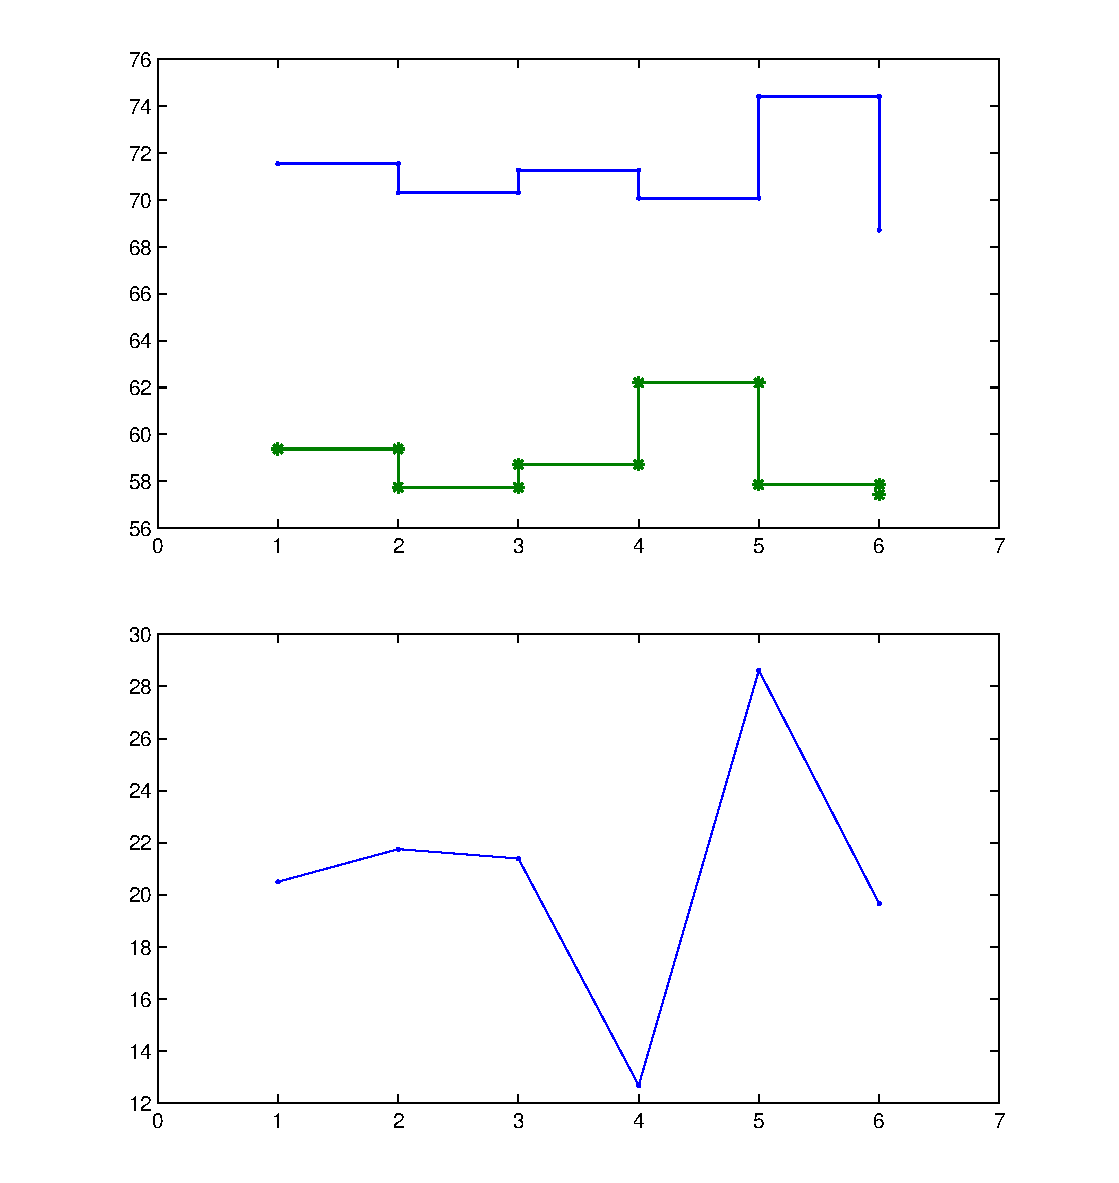
\includegraphics[scale=0.7]{9lessons.eps}}
  \caption{9\,节课打分. 上图为前后分数对比, 下图为优化率.}
  \end{figure}
  我们很惊喜的发现, 自修课之后一般都有英语课, 这样学生不但能在课上有时间复习英语默写, 取得好成绩, 也不会因此影响英语课之前课程的学习效率, 使得整张课表显得更为科学.
 \subsection{敏感度分析}
  我们发现优化率出奇的高, 所以我们对于自修课后一节课的状态进行敏感度分析. 我们选取了高一(6)班 (创新班) 以及高一(1)班 (平行班) 进行分析, 同时以原课表分数作为基准线绘制得出了如下图像:
  \begin{figure}[H]
  \centerline{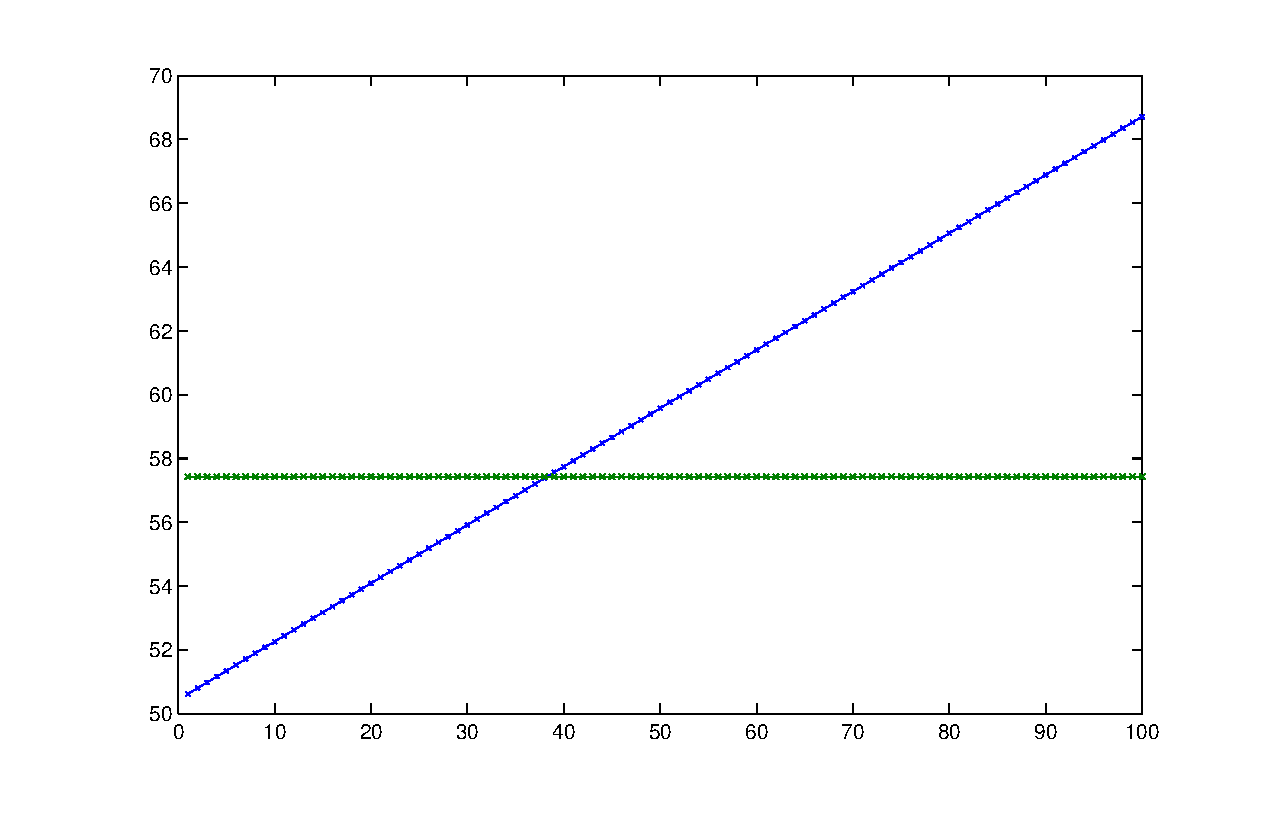
\includegraphics[scale=0.5]{seninno.eps}}
  \caption{敏感度分析: 高一(6)班 (创新班)}
  \end{figure}
  \begin{figure}[H]
  \centerline{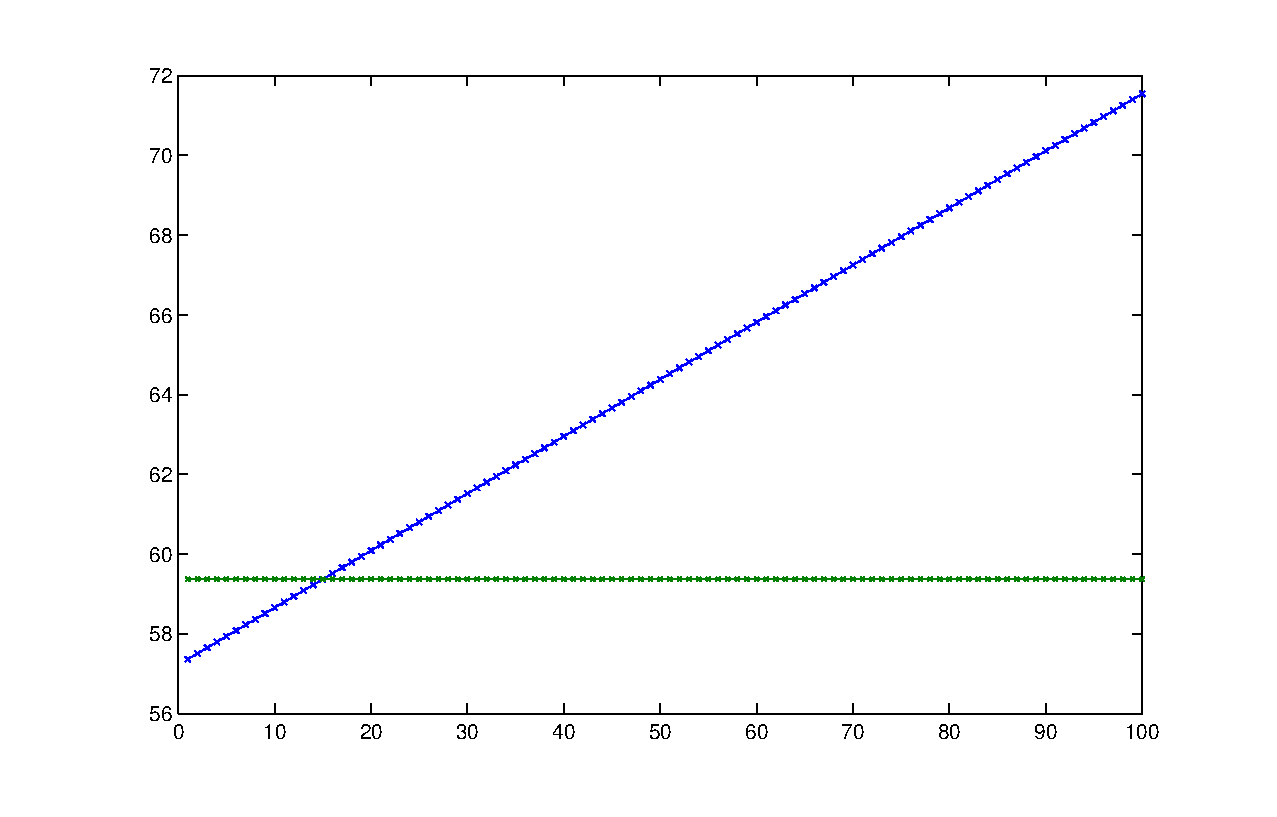
\includegraphics[scale=0.5]{sennorm.eps}}
  \caption{敏感度分析: 高一(1)班 (平行班)}
  \end{figure}
  我们可以发现高一(6)班只有当初状态分数小于\,40\%\,时才比原课表分数低, 而高一(1)班更是达到了\,15\%. 可以说\,9\,节课的优化效果还是不错的.
 \clearpage
 \subsection{新\,9\,节课想法及优化}
  我们在这里提出一种新的优化模式, 在周四下午末\,2\,节增加自修课, 其余和之前变化相同. 目的在于留出时间进行年级, 部级, 校级的活动或是比赛, 这样可以避免在中午的时间进行以上活动, 给同学们留出中午的时间. 下面是新优化的\,9\,节课课表及其打分和优化率:
  \subsubsection{高一(1)班}
   \begin{tabular}{|c|c|c|c|c|c|}
   \hline
   & \bf 星期一 & \bf 星期二 & \bf 星期三 & \bf 星期四 & \bf 星期五 \\\hline
   \bf 1 & 英语 & 语文 & 数学 & 英语 & 数学 \\\hline
   \bf 2 & 物理 & 语文 & 历史 & 数学 & 物理 \\\hline
   \bf 3 & 研究 & 音乐 & 信息 & 化学 & 地理 \\\hline
   \bf 4 & 化学 & 体育 & 信息 & 语文 & 英语 \\\hline
   \bf 5 & 语文 & 数学 & 地理 & 政治 & 语文 \\\hline
   \bf 6 & 数学 & 英语 & 英语 & 历史 & 政治 \\\hline
   \bf 7 & 活动 & 物理 & 化学 & 体育 & 班会 \\\hline
   \bf 8 & TFT  & 地理 & 特需 & 自修 & 社团 \\\hline
   \bf 9 & 拓展 & 拓展 & 特需 & 自修 & 社团 \\\hline
   \end{tabular}
  \subsubsection{高一(2)班}
   \begin{tabular}{|c|c|c|c|c|c|}
   \hline
   & \bf 星期一 & \bf 星期二 & \bf 星期三 & \bf 星期四 & \bf 星期五 \\\hline
   \bf 1 & 数学 & 物理 & 语文 & 数学 & 物理 \\\hline
   \bf 2 & 英语 & 政治 & 语文 & 化学 & 数学 \\\hline
   \bf 3 & 地理 & 化学 & 化学 & 信息 & 历史 \\\hline
   \bf 4 & 政治 & 体育 & 英语 & 信息 & 地理 \\\hline
   \bf 5 & 语文 & 英语 & 数学 & 语文 & 研究 \\\hline
   \bf 6 & 物理 & 语文 & 音乐 & 英语 & 英语 \\\hline
   \bf 7 & 活动 & 数学 & 地理 & 体育 & 班会 \\\hline
   \bf 8 & TFT  & 历史 & 特需 & 自修 & 社团 \\\hline
   \bf 9 & 拓展 & 拓展 & 特需 & 自修 & 社团 \\\hline
   \end{tabular}
  \subsubsection{高一(3)班}
   \begin{tabular}{|c|c|c|c|c|c|}
   \hline
   & \bf 星期一 & \bf 星期二 & \bf 星期三 & \bf 星期四 & \bf 星期五 \\\hline
   \bf 1 & 数学 & 英语 & 语文 & 数学 & 化学 \\\hline
   \bf 2 & 地理 & 体育 & 语文 & 英语 & 数学 \\\hline
   \bf 3 & 英语 & 政治 & 英语 & 化学 & 语文 \\\hline
   \bf 4 & 语文 & 历史 & 数学 & 研究 & 物理 \\\hline
   \bf 5 & 信息 & 数学 & 地理 & 历史 & 音乐 \\\hline
   \bf 6 & 信息 & 物理 & 物理 & 地理 & 英语 \\\hline
   \bf 7 & 活动 & 语文 & 化学 & 体育 & 班会 \\\hline
   \bf 8 & TFT  & 政治 & 特需 & 自修 & 社团 \\\hline
   \bf 9 & 拓展 & 拓展 & 特需 & 自修 & 社团 \\\hline
   \end{tabular}
  \clearpage
  \subsubsection{高一(4)班}
   \begin{tabular}{|c|c|c|c|c|c|}
   \hline
   & \bf 星期一 & \bf 星期二 & \bf 星期三 & \bf 星期四 & \bf 星期五 \\\hline
   \bf 1 & 数学 & 数学 & 英语 & 数学 & 语文 \\\hline
   \bf 2 & 物理 & 体育 & 数学 & 语文 & 语文 \\\hline
   \bf 3 & 政治 & 语文 & 政治 & 英语 & 数学 \\\hline
   \bf 4 & 活动 & 英语 & 音乐 & 历史 & 物理 \\\hline
   \bf 5 & 英语 & 物理 & 信息 & 研究 & 英语 \\\hline
   \bf 6 & 语文 & 历史 & 信息 & 地理 & 化学 \\\hline
   \bf 7 & 化学 & 化学 & 地理 & 体育 & 班会 \\\hline
   \bf 8 & TFT  & 地理 & 特需 & 自修 & 社团 \\\hline
   \bf 9 & 拓展 & 拓展 & 特需 & 自修 & 社团 \\\hline
   \end{tabular}
  \subsubsection{高一(5)班 (理科班)}
   \begin{tabular}{|c|c|c|c|c|c|}
   \hline
   & \bf 星期一 & \bf 星期二 & \bf 星期三 & \bf 星期四 & \bf 星期五 \\\hline
   \bf 1 & 英语 & 数学 & 语文 & 英语 & 数学 \\\hline
   \bf 2 & 数学 & 英语 & 语文 & 数学 & 语文 \\\hline
   \bf 3 & 化学 & 历史 & 英语 & 体育 & 地理 \\\hline
   \bf 4 & 活动 & 体育 & 政治 & 地理 & 政治 \\\hline
   \bf 5 & 物理 & 信息 & 化学 & 历史 & 化学 \\\hline
   \bf 6 & 语文 & 信息 & 物理 & 音乐 & 英语 \\\hline
   \bf 7 & 研究 & 地理 & 数学 & 语文 & 班会 \\\hline
   \bf 8 & TFT  & 物理 & 特需 & 自修 & 社团 \\\hline
   \bf 9 & 拓展 & 拓展 & 特需 & 自修 & 社团 \\\hline
   \end{tabular}
  \subsubsection{高一(6)班 (创新班)}
   \begin{tabular}{|c|c|c|c|c|c|}
   \hline
   & \bf 星期一 & \bf 星期二 & \bf 星期三 & \bf 星期四 & \bf 星期五 \\\hline
   \bf 1 & 语文 & 数学 & 数学 & 数学 & 地理 \\\hline
   \bf 2 & 语文 & 语文 & 历史 & 物理 & 英语 \\\hline
   \bf 3 & 地理 & 研究 & 自修 & 体育 & 信息 \\\hline
   \bf 4 & 活动 & 体育 & 英语 & 政治 & 信息 \\\hline
   \bf 5 & 数学 & 化学 & 物理 & 英语 & 政治 \\\hline
   \bf 6 & 物理 & 地理 & 特需 & 音乐 & 化学 \\\hline
   \bf 7 & 化学 & 英语 & 特需 & 历史 & 班会 \\\hline
   \bf 8 & TFT  & 语文 & 特需 & 自修 & 社团 \\\hline
   \bf 9 & 拓展 & 拓展 & 特需 & 自修 & 社团 \\\hline
   \end{tabular}
  \subsubsection{打分}
   \begin{table}[H]
   \centering
   \begin{tabular}{|c|c|c|c|}
   \hline
   \bf 班级 & \bf 原始分数 & \bf 优化分数 & \bf 优化率 (\%) \\\hline
   \bf 1 & 64.40172 & 59.37332 & 8.469123842 \\\hline
   \bf 2 & 63.08168 & 57.74784 & 9.236432047 \\\hline
   \bf 3 & 60.25792 & 58.71016 & 2.636272836 \\\hline
   \bf 4 & 62.92264 & 62.194548 & 1.170668529 \\\hline
   \bf 5 & 63.58474 & 57.85312 & 9.907192559 \\\hline
   \bf 6 & 61.72536 & 57.42696 & 7.484986146 \\\hline
   \end{tabular}
   \caption{新\,9\,节课打分. 平均优化率: \textbf{6.48411266\%}.}
   \end{table}
   \begin{figure}[H]
   \centerline{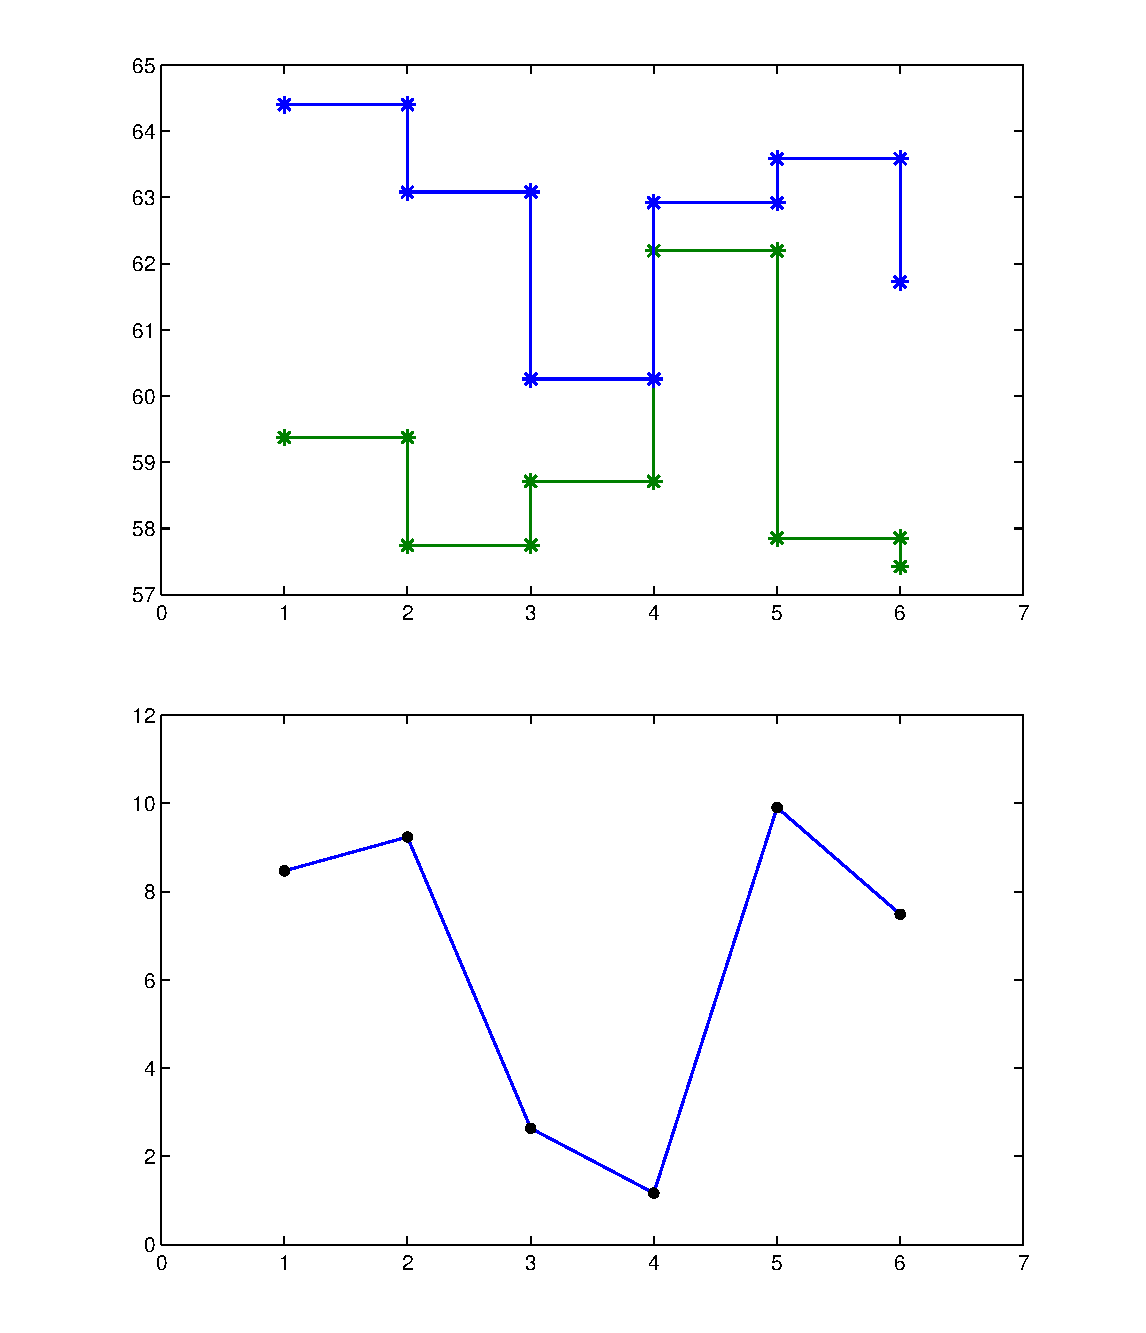
\includegraphics[scale=0.5]{new9lessons.eps}}
   \caption{新\,9\,节课打分. 上图为前后分数对比, 下图为优化率.}
   \end{figure}
\clearpage
\section{细微改动}
 我们将调整课后竞赛班的时间, 首先, 现在的吃饭时间学生们普遍反应较紧, 用餐不到位, 一来影响之后的学习效果 (饿肚子学习效率低, 边吃东西边上课学习效率更低), 二来刚吃饱饭就上课对于思考和肠胃消化多是不利的. 分析图像\,\cite{food}, 我们将竞赛班时间延后至\,17:15\,左右更为合适, 消化的情况较好, 同时提高学习的效率.
 \begin{figure}[H]
 \centerline{\begin{overpic}[scale=0.5]{food.eps}
 \put(49,4){时间}
 \put(7,35){\rotatebox{90}{消化效率}}
 \put(81,70){\colorbox{white}{\tiny 折线\qquad\quad}}
 \put(81,67.5){\colorbox{white}{\tiny 拟合曲线\quad}}
 \end{overpic}}
 \caption{食物的消化效率和时间的关系}
 \end{figure}
\clearpage
\section{结论}
 本文对于现行的\,8\,节课课表进行了优化, 通过调整每节课的顺序, 使学生的学习效率提高了约6.2\%, 之后本文又对于课表课程数目进行了调整, 通过增加自修课以及特需课等, 解决了老师上课和培训的冲突问题和学校活动的时间安排问题, 同时又增加了学生的自主学习时间 (每个班级增加了\,53\,分钟的自主学习时间).
\clearpage
\section{优缺点}
 \subsection{优点}
  \verythree 本文对于学生的学习效率进行了具体的讨论并考虑到了每节课对于之后课程的影响.\par
  \verythree 本文考虑了许多现实中的条件并将课表的打分进行了量化.
 \subsection{缺点}
  \verythree 本文没有考虑课时的调整对于课表的安排有何影响, 只是按现在课表的课时数目进行安排.\par
  \verythree 本文没有考虑到多个年级的老师冲突问题 (即部分老师即上高一, 又上其他年级).\par
  \verythree 本文对于课表的优化思路较为单一, 没有选取更多角度进行优化.\par
  \verythree 本文没有考虑到各个班级的差异, 对于课表进行差异化 (如偏重文科、理科或创新) 的安排.
\clearpage
\bibliographystyle{plain}
\bibliography{references}
\nocite{*}
\addcontentsline{toc}{section}{参考文献}
\clearpage
\begin{appendices}
\section{程序源代码}
 \renewcommand{\baselinestretch}{1}
 \hypertarget{program}{}
 \setlength{\marginparsep}{-470pt}
 \newcounter{linenum}
 \marginpar{\flushright\tt\footnotesize\color{gray}\vspace{11pt}\forloop{linenum}{1}{\value{linenum}<47}{\arabic{linenum}\\[2.5pt]}\arabic{linenum}}
 \begin{lstlisting}
 lesn=[
 1	1	6	12	2	4	5	18	18;
 2	1	14	11	5	6	19	3	10;
 2	8	19	3	4	17	17	17	17;
 2	19	4	11	7	3	13	8	1;
 6	3	9	9	7	5	15	16	16;
 ];
 zao=[1,0;1,0];
 wu=[0.8,0.2;0.8,0.2];
 zhuan(4)={[0.3,0.7;0.7,0.3]};
 zhuan(3)={[0.4,0.6;0.6,0.5]};
 zhuan(2)={[0.45,0.55;0.55,0.45]};
 zhuan(1)={[0.48,0.52;0.52,0.48]};
 aaa=[7 9 5 9 6];
 %%aaa=[7 9 7 9 6];
 bbb=[4 4 4 3 3 3 2 2 3 3 1 1 1 1];
 zhy=[6 6 6 4 4 3 2 2 3 1 1 1 1 1];
 scon=0;
 ss=0;
 score=zeros(1,100);
 for ss=1:100;
 x=0.01*ss;
 for i=1:5;
     zao=[1,0;1,0];
     wu=[0.8,0.2;0.8,0.2];
     for j=1:5;
         if lesn(i,j)==19;
             zao=[x,1-x;x,1-x];
         end;
         if lesn(i,j)~=19;
             scon=scon+zao(1,1)*zhy(lesn(i,j));
             zao=zao.*zhuan{bbb(lesn(i,j))};
         end;
     end;
     for j=6:aaa(i);
         if lesn(i,j)==19;
             wu=[x,1-x;x,1-x];
         end;
         if lesn(i,j)~=19;
             scon=scon+wu(1,1)*zhy(lesn(i,j));
             wu=wu.*zhuan{bbb(lesn(i,j))};
         end;
     end;
 end;
 score(1,ss)=scon;
 scon=0;
 end;
 \end{lstlisting}
\end{appendices}
\end{document}